\documentclass{article}

\usepackage{arxiv}

% \usepackage[style=authoryear-comp, % Citation marks as [Jef65]
%             natbib=true,      % Natbib-style cite macros \citeauthor &c.
%             hyperref=true,    % Cites in pdf are links to bib
%                               % (hyperref conf.)
%             maxnames=3,       % truncate name lists if more than 2
%                               % names appear
%             doi=false,        % no doi's
%             url=false,        % no url's
%             sortcites=false,  % do NOT sort cites in the style of the
%                               % bibliography
%             %backref=true     % insert backrefs in reference section
%             ]{biblatex}
\usepackage{mypackages}
\bibliography{~/Desktop/icloud/MyRefGlobal}
\usepackage{mycommands}

\usepackage[utf8]{inputenc} % allow utf-8 input
\usepackage[T1]{fontenc}    % use 8-bit T1 fonts
\usepackage{hyperref}       % hyperlinks
\usepackage{url}            % simple URL typesetting
\usepackage{booktabs}       % professional-quality tables
\usepackage{amsfonts}       % blackboard math symbols
\usepackage{nicefrac}       % compact symbols for 1/2, etc.
\usepackage{microtype}      % microtypography
\usepackage{cleveref}       % smart cross-referencing
\usepackage{lipsum}         % Can be removed after putting your text content
\usepackage{graphicx}
\usepackage{doi}

\usepackage{float}

% Statistical models based on LLM predictions
% LLMs fuel statistical models for full distributional predictions of human experimental data
% Large language models for full distributional predictions of human experimental data
\title{Beyond the best guess: Statistical modeling with predictors from large language models}

% Here you can change the date presented in the paper title
%\date{September 9, 1985}
% Or remove it
\date{}

\newif\ifuniqueAffiliation
% Uncomment to use multiple affiliations variant of author block
% \uniqueAffiliationtrue

\ifuniqueAffiliation % Standard variant of author block
  \author{ Michael Franke\thanks{Use footnote for providing further
		information about author (webpage, alternative
		address)---\emph{not} for acknowledging funding agencies.} \\
	Department of Linguistics\\
	University of Tübingen\\
	\texttt{michael.franke@uni-tuebingen.de} \\
	%% examples of more authors
	\And
	Polina Tsvilodub\thanks{Use footnote for providing further
		information about author (webpage, alternative
		address)---\emph{not} for acknowledging funding agencies.} \\
	Department of Linguistics\\
	University of Tübingen\\
	\texttt{polina.tsvilodub@gmail.com} \\
	\And
	Fausto Carcassi\thanks{Use footnote for providing further
		information about author (webpage, alternative
		address)---\emph{not} for acknowledging funding agencies.} \\
	Department of Linguistics\\
	University of Tübingen\\
	\texttt{fausto.carcassi@gmail.com} \\
	%% \AND
	%% Coauthor \\
	%% Affiliation \\
	%% Address \\
	%% \texttt{email} \\
	%% \And
	%% Coauthor \\
	%% Affiliation \\
	%% Address \\
	%% \texttt{email} \\
	%% \And
	%% Coauthor \\
	%% Affiliation \\
	%% Address \\
	%% \texttt{email} \\
}
\else
% Multiple affiliations variant of author block
\usepackage{authblk}
\renewcommand\Authfont{\bfseries}
\setlength{\affilsep}{0em}
% box is needed for correct spacing with authblk
% \newbox{\orcid}\sbox{\orcid}{\includegraphics[scale=0.06]{orcid.pdf}}
\author{Michael Franke, Polina Tsvilodub, Fausto Carcassi}
\affil{Department of Linguistics\\University of Tübingen\\
\texttt{[michael.franke|polina.tsvilodub|fausto.carcassi]@uni-tuebingen.de}}
\fi

% running right header
\renewcommand{\headeright}{}
% small title under big title
\renewcommand{\undertitle}{}
\renewcommand{\shorttitle}{Statistical modeling with LLM predictors}

%%% Add PDF metadata to help others organize their library
%%% Once the PDF is generated, you can check the metadata with
%%% $ pdfinfo template.pdf
\hypersetup{
pdftitle={Statistical modeling with LLM predictors},
pdfsubject={},
pdfauthor={Michael Franke, Polina Tsvilodub, Fausto Carcassi},
pdfkeywords={statistical models, language use, large language models, Bayesian data analysis, reference games},
}

\begin{document}
\maketitle

\begin{abstract}
	{\textcolor{gray}{\lipsum[1]}}
\end{abstract}


% keywords can be removed
% \keywords{First keyword \and Second keyword \and More}

\section{Motivation}
\label{motivation}

With the advent of deep neural transformer architectures \citep{VaswaniShazeer2017:Attention-is-Al}, large language models (LLMs) have become powerful technologies that excel on standard benchmarks and promise to serve as foundation models for a vast and diverse set of applications \citep{BommasaniHudson2021:On-the-opportun} \citep{DevlinChang2019:BERT:-Pre-train,ChungHou2022:Scaling-Instruc,OpenAI2023:GPT-4-Technical,TouvronLavril2023:LLaMA:-Open-and}, especially when augmented with supervised fine-tuning  \citep{ChungHou2022:Scaling-Instruc} and reinforcement learning from human \citep{StiennonOuyang2022:Learning-to-sum} or other \citep{BaiKadavath2022:Constitutional-} feedback.
Recently an increasing number of diverse applications has gone beyond using LLMs out-of-the-box, based on their single-run input-output behavior, and instead utilize LLMs as a part of a larger computational process.


\begin{itemize}
  \item tool use
  \item AutoGPT
  \item prompt-engineering
  \item structured reasoning
  \item for translation to programms \citep{WongGrand2023:From-Word-Model}
\end{itemize}

For all of these applications, it is crucial to understand what LLMs can or cannot reliable do.

\begin{itemize}
  \item benchmarks don't give us that
  \item mechanistic
  \item behavioral probing
\end{itemize}

Not yet addressed: derive full distribution over choice options and use for explanatory modeling.

\bigskip

\begin{color}{gray}
\textbf{SNIPPETS}

Recent work comparing LLMs to human choice behavior in psychological experiments has focused on whether LLMs predict patterns of human answer behavior qualitatively.
The bulk of this work looks at the answers generated by the LLMs.
In general, much less attention has been payed to whether LLMs can also make adequate \emph{quantitative predictions} that match human choice probabilities in suitable experiments.
(Notable exceptions at the interface of NLP and computational psycholinguistics (Linzen, Hu, Rabovsky \ldots).)

This work looks at whether probabilistic predictions of GTP-3.5 match human answer patterns also quantitatively.
Rather than looking at LLMs as behavior-generating black box, which we want to understand based on its input-output behvaior, we explore whether we can use LLMs as a predictive probabilistic model, or at least as a component of one, aiming to predict the full distribution of human experimental data.
\end{color}


\section{Experiment: Reference games}
\label{experiment-reference-games}

\begin{figure}
  \centering

  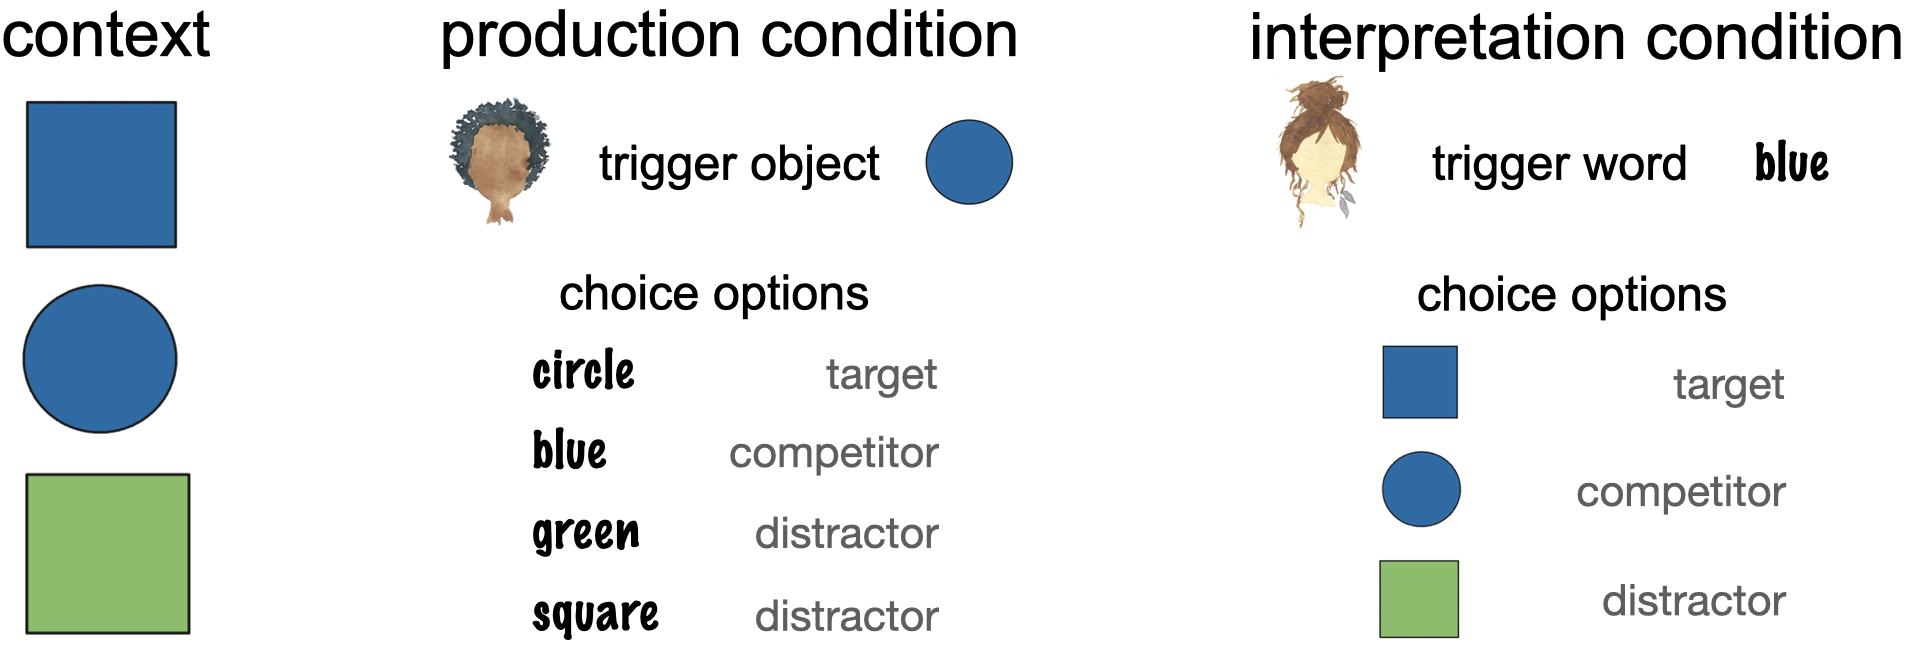
\includegraphics[width = 0.8\textwidth]{00-pics/reference-game.png}

  \caption{Structure of a reference game with human participants. Each trial consists of a set of objects, the so-called context. In production trials, participants choose a single word to describe a target object from the context. In interpretation trials, an object is selected as the likely object a trigger word referring to.}
  \label{fig:ref-game}
\end{figure}

To keep matters simple, we use an established, well-understood and austere experimental paradigm to test human decision making in abstract communicative tasks, so-called \textbf{reference games} \citep[e.g.,][]{FrankGoodman2012:Predicting-Prag,DegenFranke2013:Cost-Based-Prag,QingFranke2013:Variations-on-a,Frank2016:Rational-speech,SikosVenhuizen2021:Reevaluating-pr}.
A reference game consists of two players, a speaker and an interpreter, who jointly observe a set of objects, usually referred to as context (see Figure~\ref{fig:ref-game}).
In the \textbf{production condition}, the speaker is assigned a \emph{target object} from the context set which they have to describe to the interpreter.
In the \textbf{interpretation condition}, the interpreter observes a description, here called \emph{trigger word}, and chooses one of the objects from the context set.
The goal of the game is, for the speaker, to choose a description that enables the interpreter to choose the target object; and, for the interpreter, to guess correctly which object the speaker had in mind.

The example in Figure~\ref{fig:ref-game} is a standard case, which we will use throughout, where choices are informative about the pragmatic reasoning that decision makers engage in.
In this example, there are two features that differ across three objects (here shape and color).
One object shares both its color and shape with one other object, while the two other objects have one unique feature (e.g., being the only circle, or the only green object).
%
In a critical production trial, the target object to describe is one of the two objects with a unique feature.
The speaker has four words to choose from.
The \textbf{target utterance} is the word which uniquely describes the target object.
The \textbf{distractor utterance} is the word that is true of the target object, but also true of another object.
The other utterances, both of which are false of the target are \textbf{competitor utterance}.
%
In a critical interpretation trial, the trigger word is one that is true of two of the three objects.
If participants engage in pragmatic thought, they might reason that \emph{if} the speaker had wanted to refer to one of the two objects of which the trigger word is true (blue square and blue circle in Figure~\ref{fig:ref-game}), the speaker could have used a more informative word for exactly one of those two objects (``circle''), so they are more likely to refer to the \textbf{target object} (the blue square in Figure~\ref{fig:ref-game}).
The \textbf{competitor object} is the other object of which the trigger word is true.
The \textbf{distractor object} is the object of which the trigger word is false.

We replicated a simple reference game with human participants in which each trial instantiated the structure of the example shown in Figure~\ref{fig:ref-game}.
While previous reference games with human participants used pictorial representations of objects, and sometimes even pictorial representations of messages, we implemented a text-only version in order to be able to compare the predictions of LLMs for the exact same stimuli.
The experiment was realized as an online task using \texttt{magpie} \citep{FrankeJi:magpie:-Minimal}.\footnote{
  The code for the experiment can be found at \href{https://github.com/magpie-ea/magpie3-text-refgame}{https://github.com/magpie-ea/magpie3-text-refgame}, and a live version of the experiment can be tested at \href{https://magpie-ea.github.io/magpie3-text-refgame/}{https://magpie-ea.github.io/magpie3-text-refgame/}.
}


\subsection{Participants}
\label{participants}

A total of 302 participants were recruited via Prolific for monetary
compensation (\textsterling0.45, corresponding to roughly \textsterling 15.40 per hour).
All participants self-identified as native speakers of English.

\subsection{Materials \& design}
\label{materials-design}

We created 100 different items as stimulus material via a stochastic process.
Each item is a different textual description of a reference game with the same logical structure as the example from Figure~\ref{fig:ref-game}.
For each item, the context consisted of three objects.
Objects are defined by a triple of properties, namely a color, a shape and a texture.
For each property, there were four possible values, e.g., blue, green, red, and orange for color.
The sampled items differed in terms of the properties of the objects in the context set, and in terms of the order in which the objects and expression alternatives were presented in the text.
Figures~\ref{fig:refgame-screenshot-production} and \ref{fig:refgame-screenshot-interpretation} from Appendix~\ref{sec:scre-from-online} show example screenshots from the experiment.

\subsection{Procedure}
\label{procedure}

For each participant the experiment sampled four different items.
Participants first played two of these in the production condition, then the other two in the interpretation condition.


\subsection{Results}\label{results}

The overall distribution of choices that correspond to the target, competitor, and distractor states is shown in Figure~\ref{fig:refgame-counts} on the left.\footnote{
  The production condition actually has two distractor choices.
  Here and in the following, these are lumped together as a single category, also when modeling random errors in later models.
  This is a simplification but does not change anything of substance.}
It is interesting that the distractor options were chosen rather often.
We also see that the number of target choices is higher in the production condition than in the interpretation condition.
This is in line with previous experimental results on human reference games.
% \citep{QingFranke2013:Variations-on-a}.
For example, in previous forced-choice reference games with human participants with pictorial presentations of objects, \citet{QingFranke2013:Variations-on-a} observed the following proportions: $\tuple{0.882, 0.118, 0}$ in the production and $\tuple{0.492, 0.506, 0.003}$ in the interpretation condition (for 288 observations in each condition).

\begin{figure}
  \centering

    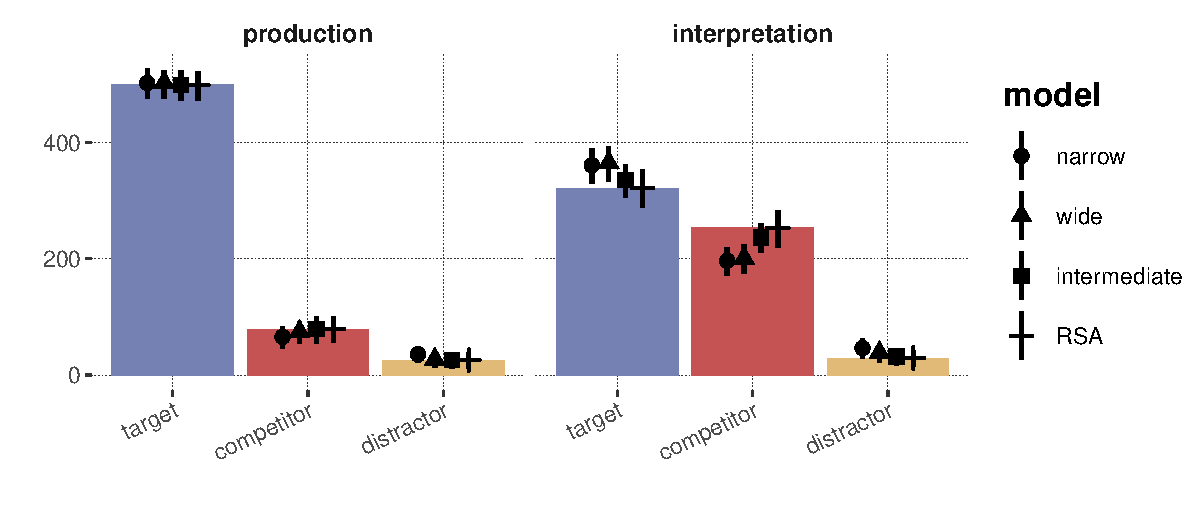
\includegraphics[width=0.9\linewidth]{00-pics/PPC-alpha-eps-model.pdf}

    \caption{Counts of choices from reference games with human participants (colored bars), with summary statistics from the posterior predictive distribution of three models (shapes and error bars).
      Shapes show the mean of the posterior predictive distributions of three models, differing in the scope of the item-level aggregation with respect to soft-maximizing and scaling.
      Error-bars show corresponding 95\% credible intervals of the posterior predictive.
    }
  \label{fig:refgame-counts}
\end{figure}

\section{LLM predictions for reference games}
\label{llm-predictions-for-reference-games}

This section explores different ways of deriving quantitative predictions from an LLM to feed into a statistical model for the human data.
For a set-up in which the task descriptions and choice options are all text-based, predictions of LLMs at the item-level can be derived as a function of the (log) probabilities assigned to the continuations corresponding to each choice option after processing the task description.
The previous literature has shown that scoring longer sequences of text for an autoregressive LLM in terms of \emph{average next-token log probabilities}, or \emph{average log-probs} for short, gives improved predictions in relevant benchmark tests \citep[e.g.,][]{BrownMann2020:Language-Models}.
Using average log-probs for each answer option as a basic item-level score, there are at least three conceivable ways of deriving condition-level predictions by averaging over item-level variation (see Figure~\ref{fig:measures-overview}).
In the following, we first describe the different options of deriving LLM-based predictor terms.
We then introduce a theoretical cognitive model for comparison.
Finally, we compare all probabilistic models based on their adequacy of explaining the human choice data.

\begin{figure}
  \centering
  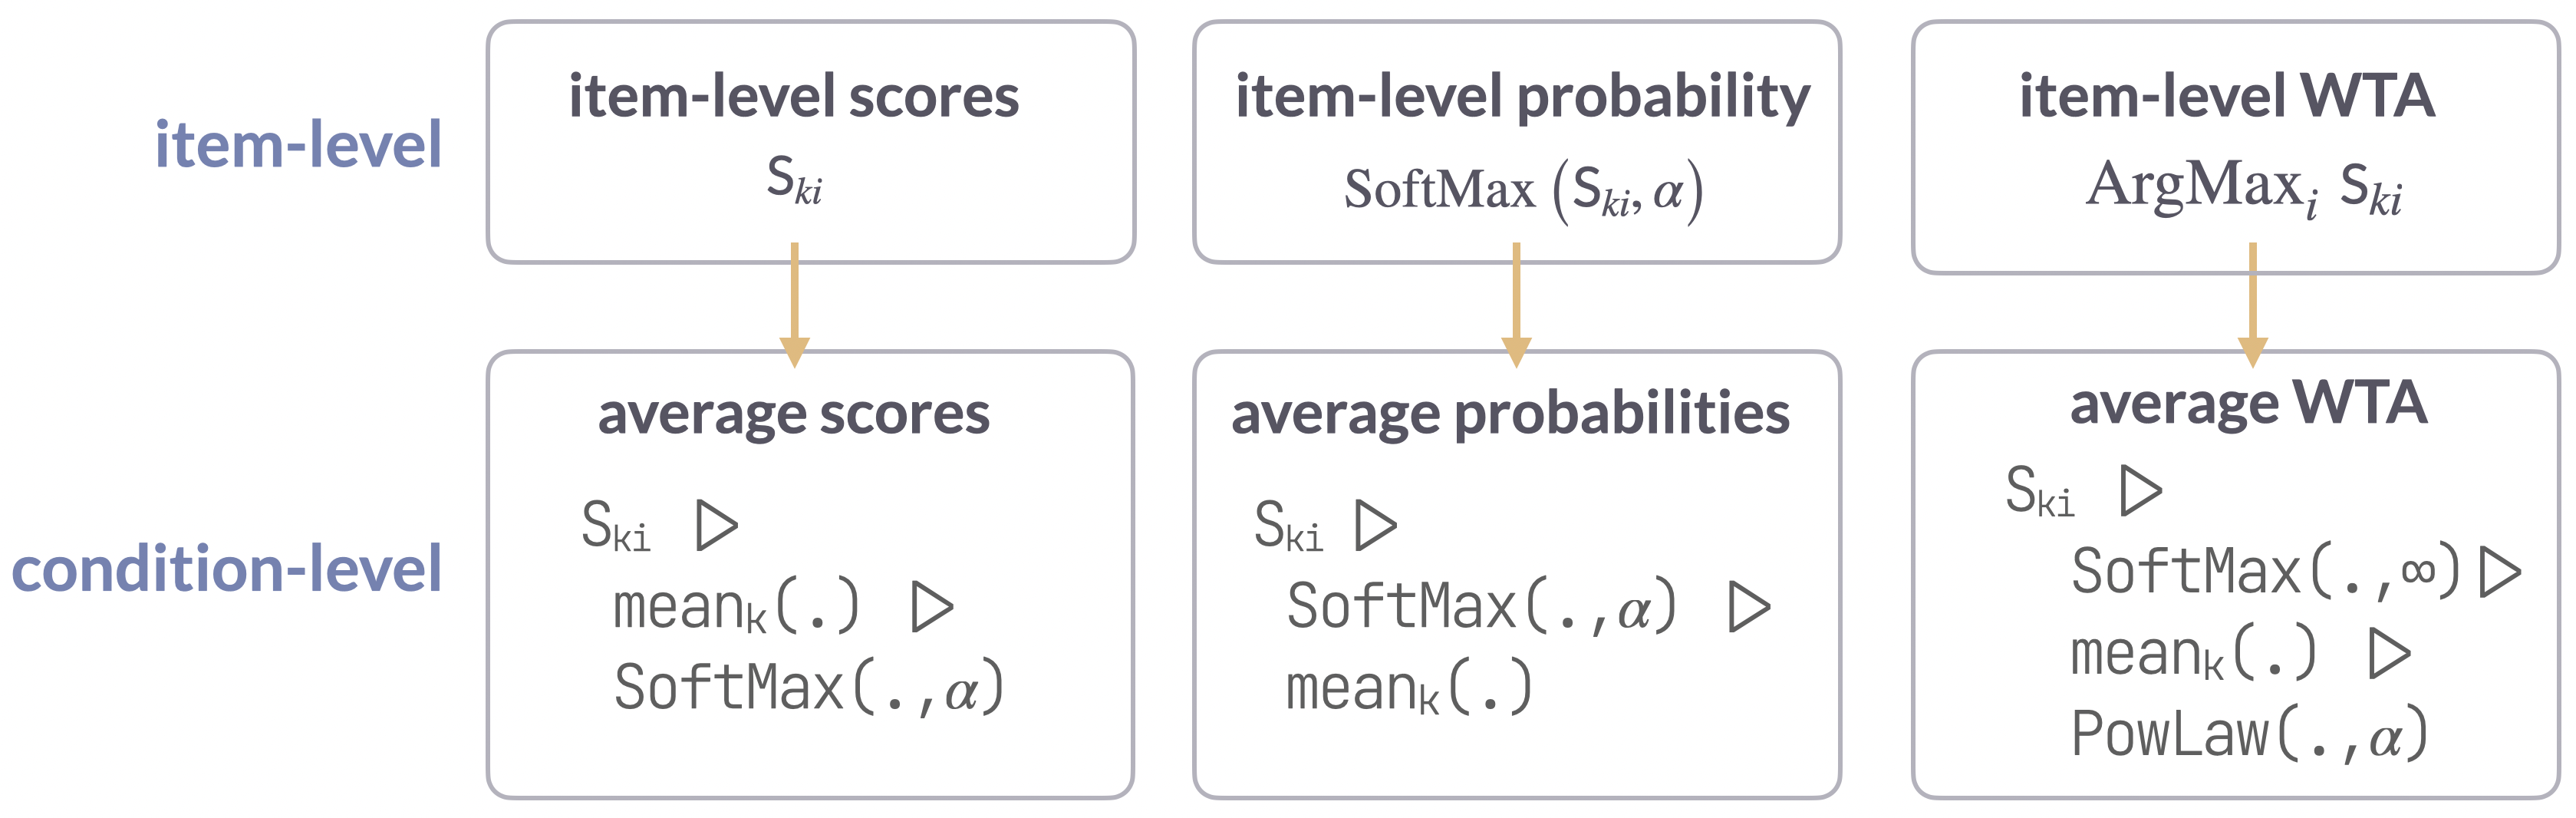
\includegraphics[width=0.9\textwidth]{00-pics/measures-overview.png}
  \caption{Schematic overview over three different approaches of obtaining condition-level predictions by aggregating over item-level scores. The basic item-level score is average next-word log probability. This can be taken as-is into averaging (narrow-scope aggregation), or first transformed from log- into probability-space, either with optimization before (wide scope) or after averaging (intermediate scope).
  The notation for the condition-level options uses pseudo-code to more clearly reflect the relevant operator scope differences (where triangles represent the pipe operator).}
  \label{fig:measures-overview}
\end{figure}

\subsection{LLM-based probabilistic predictions for forced-choice data}
\label{sec:notat--term}

Let $C$ be the experimental condition of interest (here: the production or interpretation condition).
Let \(\set{I_1, \dots I_m}\) be the multi-set of items that occurred in the human experiment for condition $C$.\footnote{
  By using a multi-set, which may contain a single task multiple times, we produce aggregate predictions for exactly the set of item that the participant group saw, which provides the most fitting counterpart to the human data.
}
Each item $I_{k}$ consists of a task description $T_{k}$ and $l$ choice options $O_{k1}, \dots, O_{kl}$, which are treated as textual continuations of the task description (see Appendix~\ref{sec:examples-items-llm} for an example).
For each item $I_{k}$, let $F(R_{l}, I_{k})$ be the choice option $O_{ki}$ that corresponds to \emph{response type} $R_{l}$ (here: target, competitor, distractor).\footnote{In the current set-up the response type ``distractor'' has two instantiations in the production condition. Since choice options are a single word in the production condition, for simplicity, we lump both of the distractor words together and treat them as a single option by taking the sum of the log-probabilities for both distractor words.}
We will define an item-level (non-normalized) score $S(O_{ki})$ for each choice option of a given item $k$, and use this to define a condition-level probabilistic predictions for response types by averaging over all items in a given condition.

\paragraph{Item-level score.}
If a choice option $O_{ki} = w$ is a single word, like in the production condition, an LLM's item-level prediction can simply be defined as the next-word log probability $\log P_{\text{LLM}} (w \mid T_{k})$.
If choice options are strings of more than one word, as in the interpretation condition, we follow the previous literature \citep[e.g.,][]{BrownMann2020:Language-Models} and define the \emph{item-level score} $S(O_{{ki}}, I_{k})$ for option $O_{ki} = w_{ki1}, \dots w_{kin}$ of item $k$, in terms of the average log-probs:
%
\begin{align*}
S(O_{ki}, I_{k}) =  \frac{1}{n} \sum_{j=1}^n \log P_{\text{LLM}} \left(w_{kij} \mid T_{k}, w_{ki1}, \dots, w_{ki(j-1)} \right)  \,.
\end{align*}
%
The item-level score of response type $R_{l}$ is $S(R_{l}, I_{k}) = S(F(R_{l}, I_{k}))$.

\paragraph{Condition-level predictions.}
Condition-level predictions are a probability distribution over response types, obtained from item-level scores $S(R_{l}, I_{k})$ by averaging over all items belonging to the relevant condition.
To map non-normalized scores $\myvec{s} = \tuple{s_{1}, \dots, s_{l}}$ to probabilities $\myvec{p} = \tuple{p_{1}, \dots, p_{l}}$ with different degrees of optimization, a common choice is the softmax function with optimality parameter $\alpha$, defined as:
%
\begin{align*}
 \text{SoftMax}(\myvec{s}, \alpha) = \myvec{p}, \text{where } p_{i} \propto \expo \left (\alpha p_{i} \right )
\end{align*}
%
The softmax function can furthermore be decomposed into a first step of mapping scores to probabilities, and subsequently reweighing probabilities via a power-law transformation:
%
\begin{align*}
  \text{SoftMax}(\myvec{s}, \alpha) & = \text{Pow}( \text{SoftMax}(\myvec{s}, 1) ; \alpha) \\
  \text{Pow}(\myvec{p} ; \alpha) & = \myvec{q}, \text{where } q_{i} \propto p_{i}^{\alpha}
\end{align*}
%
This means that there are three conceivable scope-sites for aggregating item-level information as shown in Figure~\ref{fig:measures-overview}.
Narrow-scope aggregation first aggregates the item-level scores, and then transposes the averages into (scaled) probabilities:
%
\begin{align*}
  % & \textbf{narrow-scope aggregation} \\
  & P_{n}(R_{l}, C ; \alpha) \propto \expo \left [  \alpha \ \frac{1}{m} \ \sum_{i = k}^{m} S(R_{l}, I_{k})  \right ]
    \tag*{\textcolor{gray}{[narrow-scope aggregation]}}
\end{align*}
%
Wide-scope aggregation, first transposes scores into probabilities, scales them and only aggregates over items last.
\begin{align*}
  % & \textbf{wide-scope aggregation} \\
  & P_{w}(R_{l}, C ; \alpha) \propto \frac{1}{m} \ \sum_{i = k}^{m} \frac{\expo \left( \alpha \ S(R_{l}, I_{k}) \right )}{ \sum_{l'} \expo \left( \alpha \ S(R_{l'}, I_{k}) \right )}
    \tag*{\textcolor{gray}{[wide-scope aggregation]}}
\end{align*}
%
Intermediate-scope aggregation performs item-level averaging after mapping scores onto probabilities (using softmax with $\alpha=1$), but before scaling (with a power-law transformation with variable $\alpha$):
\begin{align*}
  % & \textbf{intermediate-scope aggregation} \\
  & P_{i}(R_{l}, C ; \alpha) \propto  \left [ \frac{1}{m} \ \sum_{i = k}^{m} \frac{\expo \left( S(R_{l}, I_{k}) \right )}{ \sum_{l'} \expo \left( S(R_{l'}, I_{k}) \right )} \right ]^{\alpha}
    \tag*{\textcolor{gray}{[intermediate-scope aggregation]}}
\end{align*}

All three condition-level predictors coincide when there is only one item, of course.
For more items, wide-scope and intermediate-scope aggregation coincide when $\alpha = 1$.
In all other cases, the predictors are not guaranteed to be identical.
Conceptually, the main difference is what each measure considers to be the basic item-level unit to aggregate over.
Narrow-scope aggregation considers raw scores, not \emph{not} probabilistic predictions at the item level.
Wide-scope aggregation considers $\alpha$-optimized probabilities at the item level, which is compatible with a procedure of sampling, via softmax decoding, item-level answer options.
Similarly, intermediate-scope aggregation is also compatible with a sampling based picture, but would use pure decoding (without $\alpha$-optimization) at the item level.

\subsection{Model predictions from probabilistic pragmatics}
\label{sec:model-pred-from}

\mf{todo: briefly describe RSA; maybe include matrices as figure?}


\subsection{Model fitting, criticims \& comparison}
\label{sec:model-fitting}

Parameterized predictions $P_{m}(R_{l}, C ; \alpha_{c})$ for models $m \in \set{n,w,i,p}$ can be assessed in the light of the empirical data from human participants with the usual tools of Bayesian data analysis \citep[e.g.][]{GelmanCarlin2014:Bayesian-Data-A,McElreath2016:Statistical-Ret,Lambert2018:A-Students-Guid}.
For each condition $C$ (production and interpretation), each model has a free optimality parameter $\alpha_{c}\sim \text{log-Normal}(0.5,1)$ with a log-Normal prior.
We also assume that each model has one epsilon parameter per condition, $\epsilon_{c}$, which accounts for random errors in the human data via Laplace smoothing, with a prior $\epsilon_{c} \sim \text{Beta}(1,5)$ favoring small values.
The resulting likelihood function for model $m$ and data from condition $C$ is a multinomial distribution with central predictor for response $R_{l}$ given by:
%
\begin{align*}
  P(R_{l}) \propto P_{m}(R_{l}, C; \alpha_{c}) +  \epsilon_{c}
\end{align*}

Using Stan \citep{Team2023:The-Stan-Core-L} for Bayesian inference, we obtain estimates of posterior credible values of each $\alpha_{c}$ and $\epsilon_{c}$ for each model.
The usual Bayesian summary statistics for posteriors over model parameters are shown in Figure~\ref{fig:posterior-stats}.

\begin{figure}
  \centering

  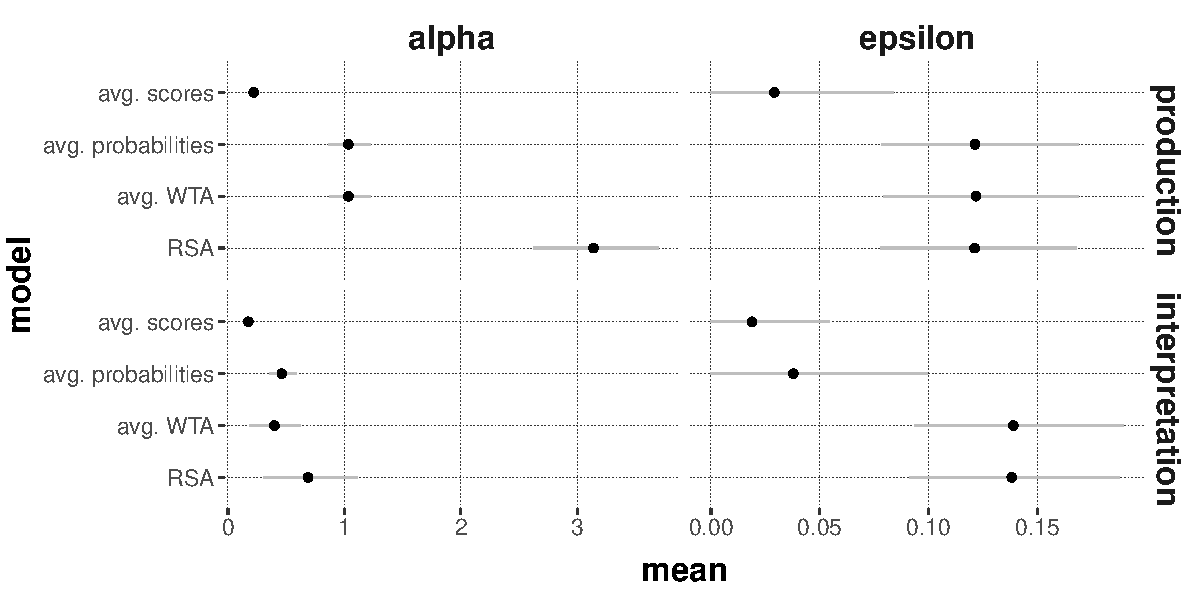
\includegraphics[width=0.9\linewidth]{00-pics/posterior-stats.pdf}

  \caption{
    Summary statistics of posterior samples.
    Black dots show means of the posterior samples, gray lines indicate 95\% credible intervals.
  }
  \label{fig:posterior-stats}
\end{figure}

To assess goodness-of-fit, Figure~\ref{fig:refgame-counts} shows summary statistics (means and 95\% credible intervals) for each model's posterior predictive distribution, i.e., the model's predictions about data of the same size and structure as the training data.
As a minimal bar, we would require a model trained on observed data $D_{\text{obs}}$ to not be surprised by $D_{\text{obs}}$.
Figure~\ref{fig:refgame-counts} shows that only the intermediate-scope model passes this ``visual posterior predictive check'' for both conditions; the other two models both overpredict the target choice rate and underpredict the competitor choice rate.
To corroborate the visual impression, Table~\ref{tab:Bppp-values} shows sample-based estimates of Bayesian posterior predictive $p$-values, using likelihood of the observed data as a test statistics.
These values approximate the probability that a model trained on $D_{\text{obs}}$ would predict future data of the same size and format that is at least as unlikely as the data $D_{\text{obs}}$ itself.
Low values therefore indicate that the trained model would be highly surprised by the data it was trained on; an indication that it failed to capture something essential about the training data.
Consequently, the results from Table~\ref{tab:Bppp-values} suggest that the narrow-scope model fails on the interpretation data, and is at most borderline on the production data; that the wide-scope model is able to reproduce the production data, but fails on the interpretation data; and that only the intermediate-scope model is able to fully recover the data from both conditions.

\begin{table}[ht]
\centering

\begin{tabular}{lrr}
  \toprule
  model        & production & interpretation \\ \midrule
  narrow       & 0.05       & 0.00 \\
  wide         & 0.51       & 0.00 \\
  intermediate & 0.49       & 0.26 \\
  RSA          & 0.50       & 0.52 \\
  \bottomrule \\
\end{tabular}

\caption{Sample-based estimates of Bayesian posterior predictive $p$-values for each model and each condition, based on likelihood of the observed data as test statistic.}
\label{tab:Bppp-values}
\end{table}

A first important conclusion from these results is that there is at least one model with predictors based on LLM-measures, namely the intermediate-scope model, which is able to recover the patterns in the data.
In other words, there is a way of deriving predictor values for condition-level forced-choice probabilities from an LLM such that, when fed into a common linking function (here with parameters $\alpha$ for optimization and $\epsilon$ for random error), the human choice probability can be reconstructed faithfully in its entirety.
On the other hand, another important lesson from this exploration is that not all ways of deriving condition-level predictions by averaging over item-level variation are equally good.
Some approaches clearly fail basic checks for statistical goodness-of-fit.


\bigskip

Next, todo:

\begin{itemize}
  \item non-triviality of intermediate-scope model
  \item predicting item-level data
\end{itemize}


\newpage

\textcolor{red}{from here on: deprecated}


\subsection{Vanilla predictions}
\label{sec:vanilla-predictions}

Since the reference game descriptions and choice options are all text-based, probabilities for discrete-choice predictions of LLMs can be defined as a function of the probabilities assigned to the continuations corresponding to each choice option after processing the game description.
Concretely, consider either the production or the interpretation case (the case is entirely parallel) and let \(\set{I_1, \dots I_m}\) be the multi-set of items that occurred in the human experiment.
By using a multi-set, which may contain a single task multiple times, we produce aggregate predictions for exactly the set of tasks that the participant group saw and so provides the most fitting counterpart to the human data.
Each item $I_{k}$ consists of a task description $T_{k}$ and three or four choice options $O_{k1}, \dots, O_{kl}$, which are treated as textual continuations of the task description (see Appendix~\ref{sec:examples-items-llm} for an example).

If a choice option $O_{ki} = w$ is a single word, like in the production condition, an LLM's prediction can simply be defined as the (normalized) next-word probability $P_{\text{LLM}} (w \mid T_{k})$.
But choice options can be strings of more than one word in the interpretation condition.
The previous literature has shown that scoring longer sequences of text for an autoregressive LLM in term of \emph{average next-token log probabilities} gives improved predictions in relevant benchmark tests \citep[e.g.,][]{BrownMann2020:Language-Models}.

We therefore define the conditional probability of producing $O_{ki} = w_{ki1}, \dots w_{kin}$ after task description $T_{k}$ in terms of average surprisal \mf{fix formula; conditioning on whole sequence not just last word}:
%
\begin{align*}
P(O_{ki} \mid T_{k}) \propto \expo \left [  \frac{1}{n} \sum_{j=1}^n \log P_{\text{LLM}} \left(w_{kij} \mid T_{k}, w_{ki(j-1)} \right) \right ] \,,
\end{align*}
%
where the normalization is over the different choice options $O_{k1}, \dots, O_{kl}$.
Notice that this definition in terms of ``log-average-exp'' reduces to simple next-word probability if $O_{ki}$ has only one word.


Finally, we determine the non-normalized probability score $S(R_{l})$ of a \emph{response type} $R_{l}$ (target, competitor, or distractor), by averaging, over all items $k$, the probabilities $P(O_{ki} \mid T_{k})$ of all choice options $O_{ki} \in F(R_{l}, I_{k})$ that correspond to this type in item $I_{k}$:
%
\begin{align*}
S(R_{l}) = \frac{1}{m} \sum_{k=1}^{m} \sum_{O_{ki} \in F(R_{l}, I_{k})} P(O_{ki} \mid T_k)\,.
\end{align*}
%
Finally, the model's \textit{vanilla predictions} are obtained by normalizing these scores:
%
\begin{align*}
\text{Prediction}(R_{l}) = \frac{S(R_{l})}{\sum_{l'} S(R_{l'})}\,.
\end{align*}
%
The vanilla predictions obtained from GPT-3.5 in this way are shown on the right-hand side in Figure~\ref{fig:refgame-counts}.




\subsection{Adding a link function: the \(\alpha\)-model}
\label{adding-a-link-function-the-alpha-model}

% source code (legacy) showing that temperature applies /before/ softmax of logits to probs https://huggingface.co/transformers/v3.1.0/_modules/transformers/generation_utils.html


On the surface, the LLM predictions show a similar ordinal pattern as the human data.
The target option is preferred over the competitor, which is in turn preferred over the distractor option(s).
Moreover, the amount of target choices is higher in the production condition than in the interpretation condition.
However, the LLM predictions have lower entropy than the distribution of the human answers.
The LLM prediction could be said to be more ``optimized'', having far fewer distractor choices and a higher ratio of target choices than the human data.

In statistical modeling, a standard way to capture degrees of variation around a predictor of central tendency is to introduce a suitable parameterized link function.
Similarly, a common decoding strategy for causal LLMs is to use softmax with non-trivial optimization parameter $\alpha$ when transforming the model's latent logits into probabilities.
Expressed in terms of probabilities, not logits, this is equivalent to using a power-law link function \citep{WorthyMaddox2008:Ratio-and-Diffe} with variable parameter \(\alpha \ge 0\), so that the $\alpha$-model's predictions are defined as:

\[\text{Prediction}(R_{l}, \alpha) = \frac{P(R_{l})^\alpha}{\sum_{l'} P(R_{l})^\alpha}\]

The predictions of the previous vanilla model are then a special case, assuming a fixed \(\alpha =1\).

Using Stan \citep{Team2023:The-Stan-Core-L} for Bayesian inference, we obtain estimates of posterior credible values of \(\alpha\), once for the production data and the model's predictions for the production condition, and once for the interpretation side.
In both cases, the model uses a single \(\alpha\) with a log-normal prior, \(\alpha \sim \text{log-Normal}(0.5,1)\) and the obvious multinomial likelihood function.
The usual Bayesian point and interval summary statistics for the two inferences are: \mf{insert proper table with reproducible numbers}

\begin{verbatim}
# A tibble: 3 x 4
  Parameter        `|95%`    mean `95%|`
  <chr>             <dbl>   <dbl>  <dbl>
1 production        0.343  0.402  0.459
2 interpretation    0.348  0.414  0.478
3 diff. prod-inter -0.101 -0.0124 0.0709
\end{verbatim}

We see that only values for \(\alpha\) below 1 are credible, which is in line with the previous observation that the human data distribution is more entropic than the vanilla model predictions.
The table also shows posterior summary statistics for a vector of derived samples, capturing the difference between estimated values for $\alpha$ between conditions.
These differences are not credibly different from zero, suggesting that the same \(\alpha\) parameter might be used for both production and interpretation cases (at least for the data at hand).

Figure~\ref{fig:PPC-alpha-model} shows the posterior predictive distributions from the two model fits.
The colored bars show the observed counts.
The black dots are the means of the posterior predictives and the black bars given the 95\% HDI of the posterior predictive distribution.
The data observations lie inside the posterior predictive 95\% HDI for the interpretation condition, suggesting that the fitted model would predict data that looks similar to what the model was condition on.
For the production data, on the other hand, this is not the case.
Even with the ability to fit \(\alpha\) to the data, the model is not able to reproduce the observed pattern in the data.

\begin{figure}[t]
  \centering

  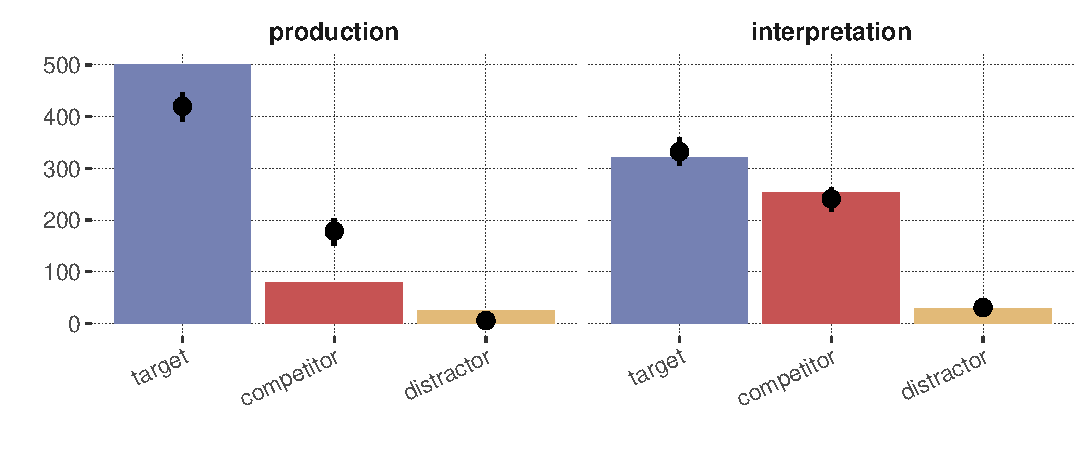
\includegraphics[width = 0.9 \textwidth]{00-pics/PPC-alpha-model.pdf}

  \caption{(Visual) posterior predictive checks for the $\alpha$-model.
    The bars show the observed counts for each category.
    Black dots are means of the posterior predictive distribution.
    Black lines indicate 95\% HDIs.
  }
  \label{fig:PPC-alpha-model}
\end{figure}


Intuitively, there are two reasons for the model's failure on production data.
First, since the model predicts a very low rate of distractor choices, we would need a rather low \(\alpha\) to increas this probability.
But, second, for low-ish values of \(\alpha\), the model cannot predict the large probability ratio in favor of target choice over competitor choices.
In sum, the model is unable to capture the quantitive patter (i.e., the set of probability ratios among choice options) adequately for the production case.

\mf{maybe include: (i) posterior predictive \(p\)-value; (ii) comment that doing soft-max on probabilities (not log-probs) is a far worse model}

\subsection{Adding noise: the \(\alpha \epsilon\)-model}
\label{sec:adding-noise-the-alpha-epsilon-model}

The $\alpha$-model's  failure to predict the human production is due, at least in part, to under-predicting the rate at which human participants selected the distractor.
But a human selection of a distractor is, most naturally, explained as an error anyway.
In experimental modeling work, it is not uncommon to include the possibility that some participants might be random guessers, but to use the data to infer the extent of guessing in the population \citep{LeeWagenmakers2013:Bayesian-Cognit}.
We therefore extent the previous $\alpha$-model with another parameter \(\epsilon \sim \text{Beta}(1,3)\), indicating the proportion of random guesses in the data set.
The predictions of the $\alpha-\epsilon$-model are defined as:

\begin{align*}
  \text{Prediction}(o_i, \alpha, \epsilon) = (1-\epsilon) \ \text{Prediction}(o_i, \alpha) + \epsilon \ \tuple{\frac{1}{3}, \frac{1}{3}, \frac{1}{3}}
\end{align*}

Summary statistics for the Bayesian posterior are shown in the table below \mf{insert label and ref}.
We see that \(\alpha\) now has higher estimates for the production model, because \(\epsilon\)-errors can help explain the distractor choices.
The \(\alpha\) estimated for the production data is now credibly higher than for the interpretation data, which makes sense, given that the production condition is intuitively easier.
There is no credible difference in estimated \(\epsilon\) between production and interpretation model.
\mf{insert proper table with reproducible numbers}

\begin{verbatim}
# A tibble: 6 x 5
  Parameter     `|95%`   mean `95%|` condition
  <chr>          <dbl>  <dbl>  <dbl> <chr>
1 alpha      0.865     1.04   1.24   production
2 epsilon    0.0306    0.0498 0.0705 production
3 alpha      0.362     0.483  0.619  interpretation
4 epsilon    0.0000116 0.0293 0.0657 interpretation
5 alpha      0.317     0.561  0.784  diff. prod-inter
6 epsilon   -0.0246    0.0205 0.0603 diff. prod-inter
\end{verbatim}

\begin{figure}[t]
  \centering

  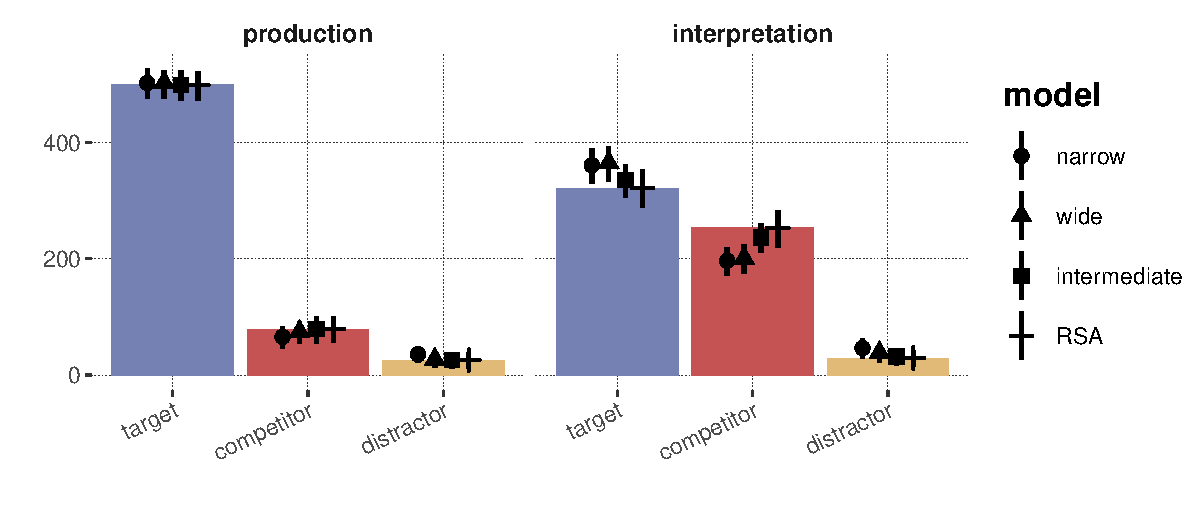
\includegraphics[width = 0.9 \textwidth]{00-pics/PPC-alpha-eps-model.pdf}

    \caption{(Visual) posterior predictive checks for the $\alpha\epsilon$-model.
    The bars show the observed counts for each category.
    Black dots are means of the posterior predictive distribution.
    Black lines indicate 95\% HDIs.
  }

  \label{fig:PPC-alpha-eps-model}
\end{figure}

Figure~\ref{fig:PPC-alpha-eps-model} shows the posterior predictive checks for the \(\alpha\epsilon\)-model.
When accommodating for an \(\epsilon\) chance of random error, the LLM-based models do not fail the visual check: once conditioned on the data, they are no longer surprised by it.
This may be a low bar to pass, but it is nonetheless reassuring that probabilistic predictions obtained from an LLM can serve as input to a probabilistic model predicting quantitative patterns in human choice data.

Moreover, it is not a trivial achievement to capture the human response patterns with an $\alpha\epsilon$-model.
It may seem that, given the freedom to adjust optimization $\alpha$ and random guessing rate $\epsilon$, it is possible to explain \emph{any} data observation.
But this is not so.
Figure~\ref{fig:prediction-range} shows the range of predictions that the $\alpha\epsilon$-model is, in principle, capable of making (for the whole possible range of \(\alpha\) and \(\epsilon\) values, disregarding Bayesian priors).
There are ranges of parameter values which the model does not explain for the vanilla LLM predictions at hand.
For example, the model does not predict well cases where the number of competitor choices is almost as high as the number of target choice, as would be the case if participants would consistently \emph{not} engage in pragmatic reasoning.


\begin{figure}[t]
  \centering

  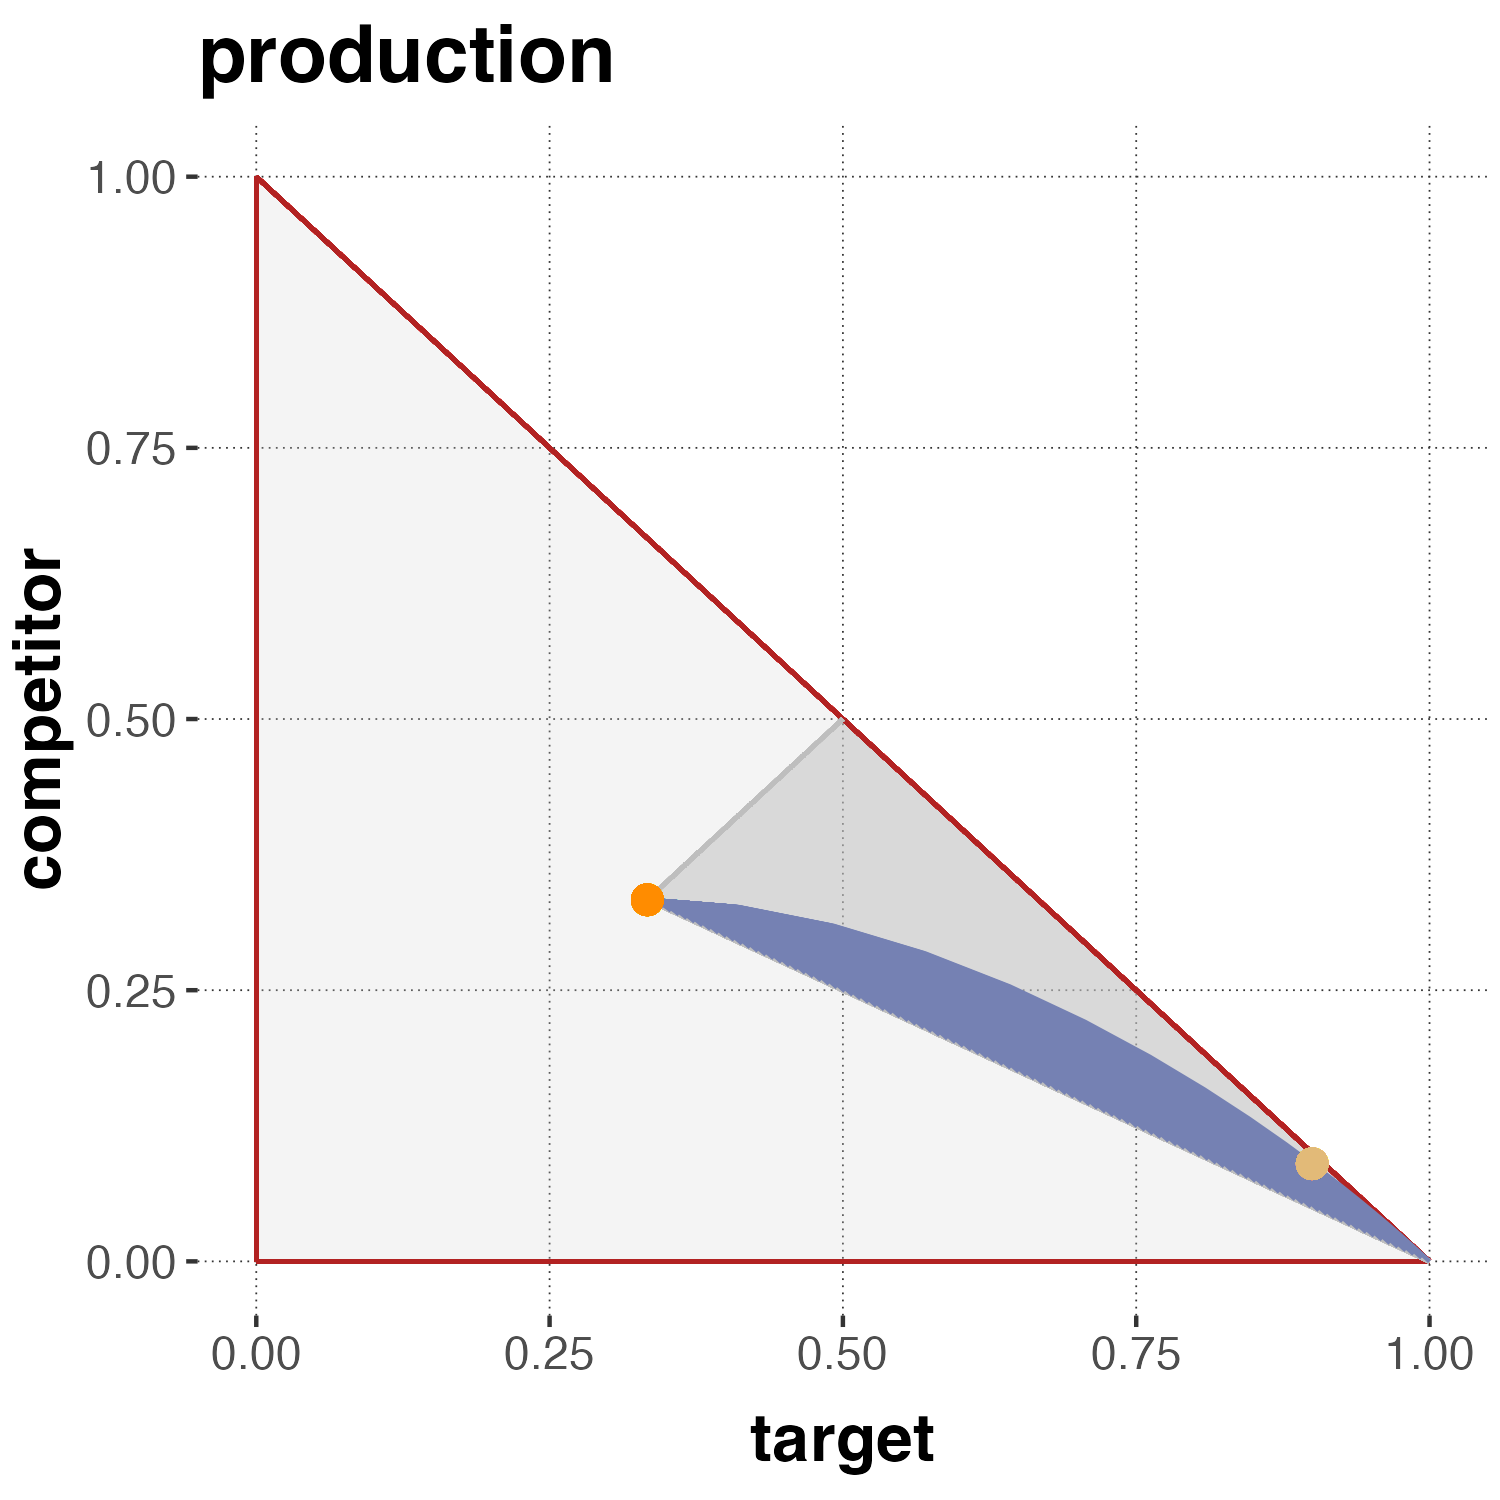
\includegraphics[width=0.45\textwidth]{00-pics/prediction-range-prod.png}
  %
  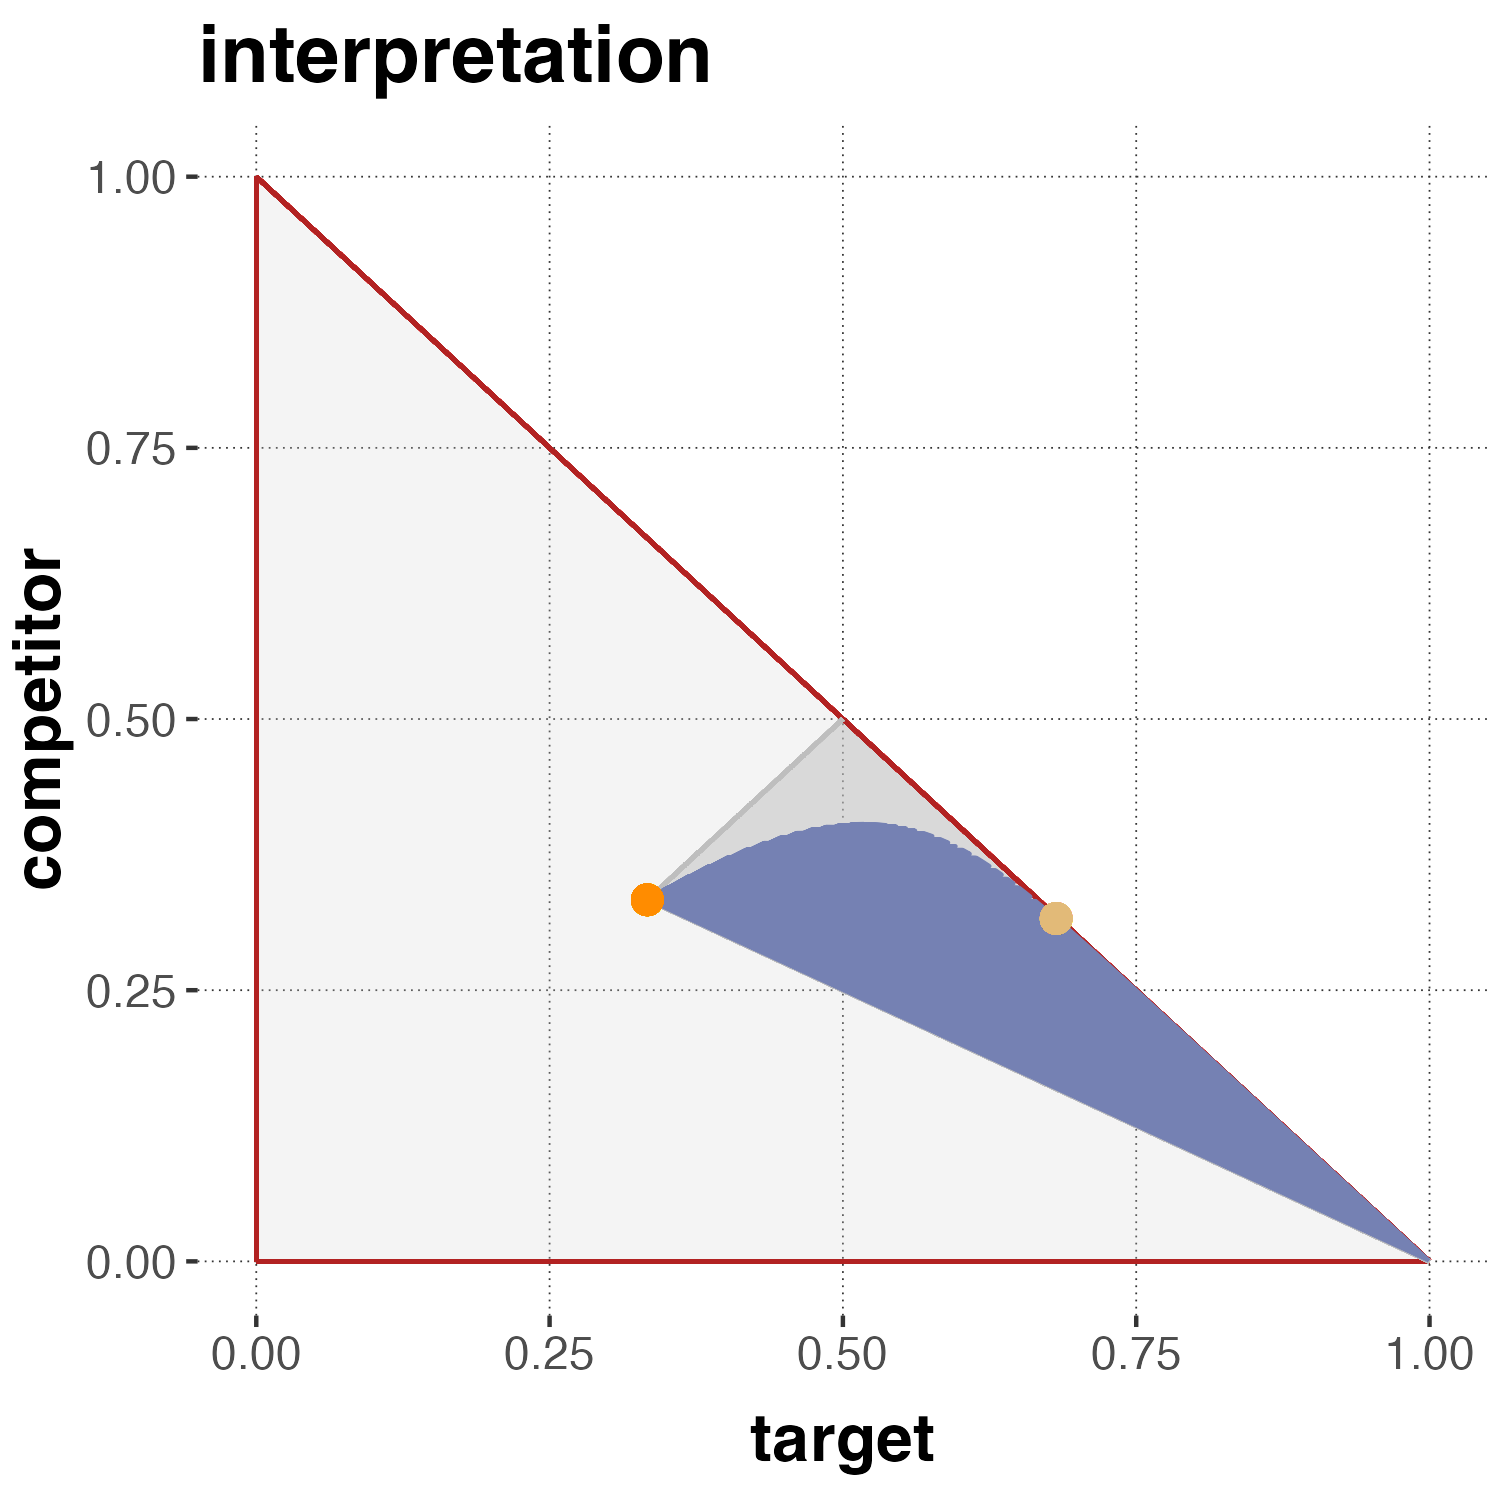
\includegraphics[width=0.45\textwidth]{00-pics/prediction-range-inter.png}

  \caption{
    Range of predictions the \(\alpha\epsilon\) model makes for any pair of parameter values under the given vanilla LLM predictions.
    The light gray triangle with the red boundary is the probability simplex, i.e., the space of all possible 3-place probability vectors.
    The darker gray area in gray boundary lines is the subspace that is compatible with the ordering that target probability is bigger than competitor probability, which in turn is bigger than distractor probability.
    The blue area is the subspace of predictions achievable under the $\alpha\epsilon$-model.
    The orange dot in the middle is the ``Laplace point'' of equal probability for all three options, which the model predicts for $\alpha=0$ or $\epsilon=1$.
    The yellow dot is the vanilla LLM prediction.
  }
  \label{fig:prediction-range}
\end{figure}


\newpage
\mf{FIRST IMPROVED DRAFT UP TO HERE}

\newpage

\section{Item-level variation}
\label{sec:item-level-variation}

The ability to predict a population average is useful for applications, and may also be theoretically insightful.
Nevertheless, averages over item- or individual-level variation can also be misleading \citep[e.g.,][]{StanovichWest2000:Individual-diff,EstesMaddox2005:Risks-of-Drawin,HaafRouder2019:Some-do-and-som}.
It is difficult to conceive of how an LLM could make genuine individual-level predictions (but see the discussion Section~\ref{conclusion}).
What an LLM does offer is differential predictions for item-level variation.
This section therefore explores this kind of variation in both human data and model predictions.
% There are essentially two potentially interesting sources of such variation.
% For one, prior experimental work suggests that human choices may be affected by which features are relevant for solving the task \citep[e.g.][]{QingFranke2013:Variations-on-a}.
% For another, the order of presentation of choice alternatives may affect LLM predictions \mf{references for systematic ordering effects?}.

The vanilla LLM predictions show item-level variance along at least two dimension: task-relevant features and ordering.
Figure~\ref{fig:feature-set-variation} shows the variation of vanilla LLM predictions across different trials, arranged by \textbf{feature sets}, which is a pair consisting of the target feature and the nuisance feature.
The \textbf{target feature} is the feature (color, shape or texture) that should be selected in the production condition and that the trigger word in the interpretation condition is an instance of.
For the example in Figure~\ref{fig:ref-game}, the target feature is color.
The \textbf{nuisance feature} is the feature whose level all objects share, so that it can, strictly speaking, be completely ignored.
For the example in Figure~\ref{fig:ref-game} the nuisance feature would be texture, because all objects share the value of that feature (in this case, no texture at all).
Figure~\ref{fig:feature-set-variation} shows that, when \textbf{color} is the target feature and \textbf{texture} is the nuisance feature, the models' predictions are consistently close to one in the production condition.
But for the feature set \textbf{shape-texture}, the model may assign an almost zero probability to the target choice.

\begin{figure}
  \centering
  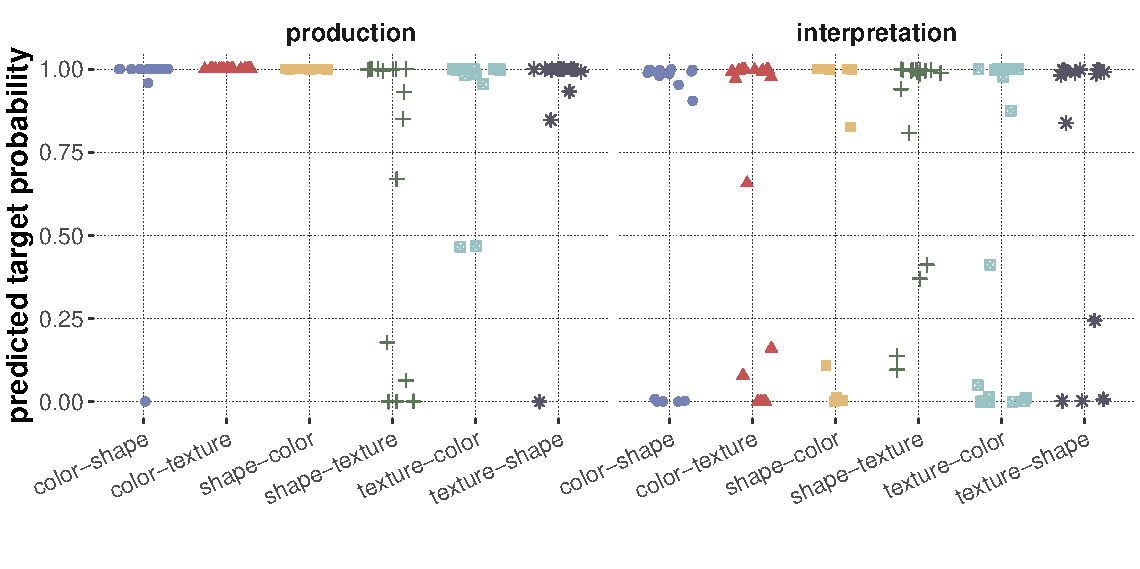
\includegraphics[width=0.9\textwidth]{00-pics/feature-set-variation.pdf}
  \caption{
    Variation in vanilla target choice prediction based on different feature sets.
    Each point in the plot represents the predicted probability of choosing the target for a given trial, split by production and interpretation condition, as well as based on which features are relevant for the task.}
  \label{fig:feature-set-variation}
\end{figure}

\bigskip

Likewise, the LLM's predictions seem to depend on the order of the choice options.
This effect is less pronounced for the production condition, as shown in the following figure (where a sequence like \texttt{[t,d,c,d]} represents a context in which the target option was presented first, then the first distractor, than the competitor and finally the second distractor).

\begin{figure}
  \centering

  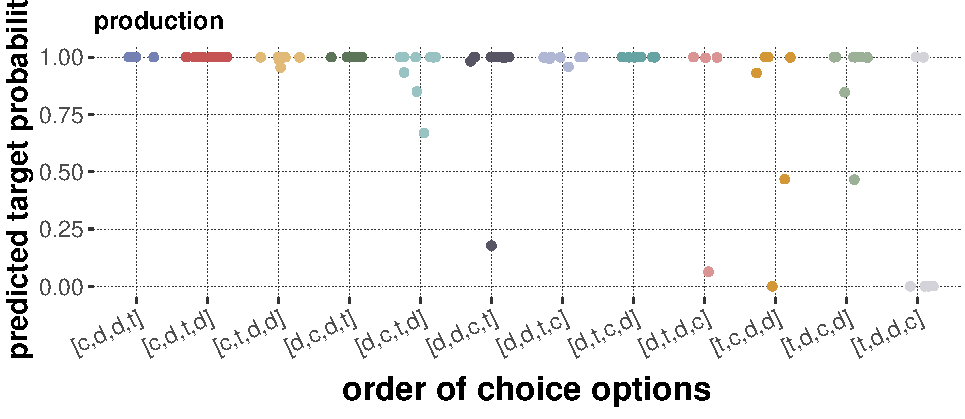
\includegraphics[width = 0.575\textwidth]{00-pics/order-variation-production.pdf}
  \hfill
  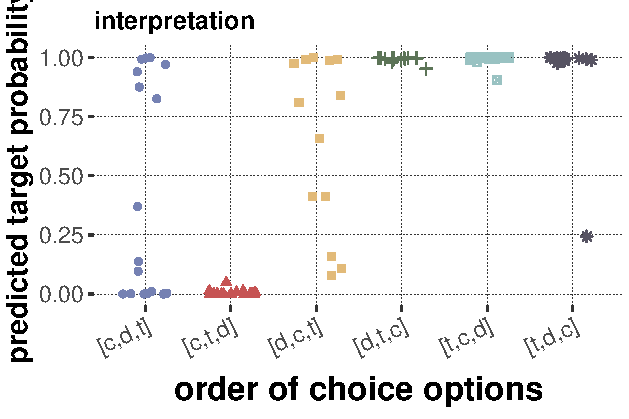
\includegraphics[width = 0.375\textwidth]{00-pics/order-variation-interpretation.pdf}

  \caption{order-variation production}
  \label{fig:order-variation-production}
\end{figure}

The effect is more pronounced for the interpretation condition. For example instances of the ordering \texttt{[c,t,d]} are assigned very low target probabilities.

% \begin{figure}
%   \centering
%   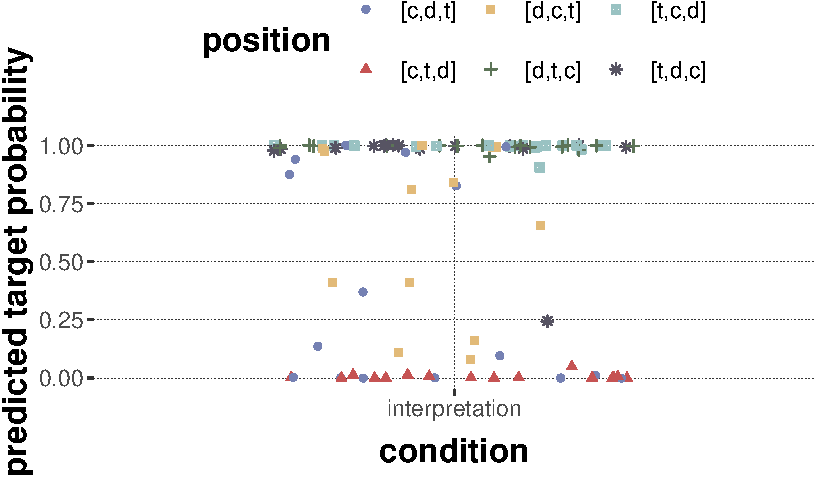
\includegraphics{00-pics/unnamed-chunk-7-1.pdf}

%   \caption{order-variation-interpretation}
%   \label{fig:order-variation-interpretation}
% \end{figure}

This demonstrates that the model's predictions are quite sensitive to differences in the context, such as the kinds of features that matter for the language task, or the order of presentation of the choice options.
The questions to be asked is therefore: do we see similar patterns also in the human data?; or should we conceive of LLMs as predictors only after aggregating over ``spurious contextual elements'' like order of presentation of alternatives?

\subsection{Effects of relevant features}

We first investigate whether the features relevant for the communicative
task have an influence on human choice behavior, and whether the LLM
predictions specific to each level of \texttt{feature\ set} yield
adequate predictions for the human data.

\hypertarget{human-data}{%
\subsubsection{Human data}\label{human-data}}

First, here are the choice counts for the human data broken up by
\texttt{feature\ set}, starting with the production condition:

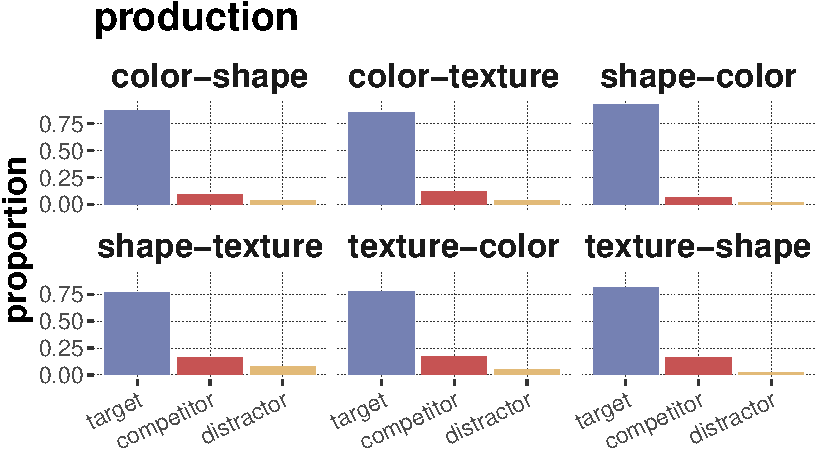
\includegraphics{00-pics/human-data-counts-per-featureSet-1.pdf}

There are some slight numerical differences, but maybe not too
noteworthy. To test whether differences for different features matter to
human answer behavior in the production task, we ran a Bayesian logistic
regression and checked whether the estimated proportions for conditions
with, respectively, the highest (\texttt{shape-color}) and lowest
observed target choice proportion (\texttt{shape-texture}) are credibly
different. We find no credible difference. This suggests that human data
has no noteworthy systematic variation based on which features are
relevant for the production task.

\begin{verbatim}
Outcome of comparing groups:
 * higher:  feature_set == "shape-color"
 * lower:   feature_set == "shape-texture"
Mean 'higher - lower':  0.3262
95% HDI:  [ -0.2583 ; 0.9392 ]
P('higher - lower' > 0):  0.859
Posterior odds:  6.092
\end{verbatim}

The picture for the interpretation task looks different. There are
conditions where the target is clearly chosen more frequently
(\texttt{shape-color}), but others where the modal choice is the
distractor (\texttt{color-texture}).

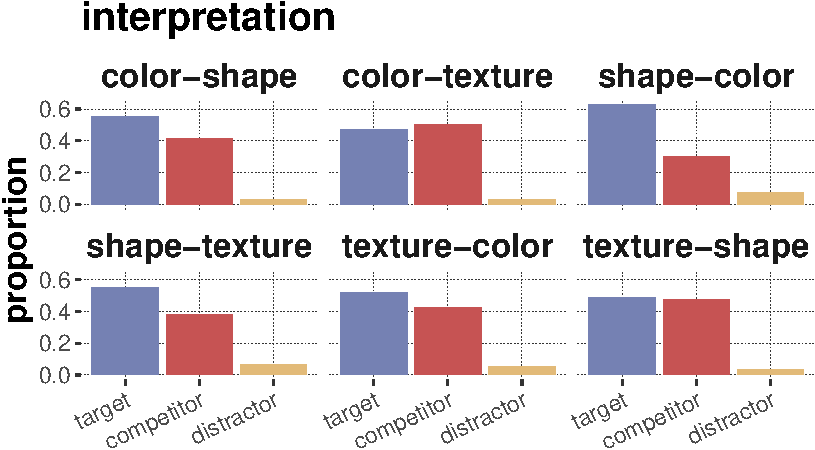
\includegraphics{00-pics/human-data-counts-per-featureSet-interpretation-1.pdf}

To test whether these differences are noteworthy, we ran another a
Bayesian logistic regression comparing the estimated proportions for
conditions with, respectively, the highest (\texttt{shape-color}) and
lowest observed target choice proportion (\texttt{color-texture}).
Indeed, it turns out that they are credibly different.

\begin{verbatim}
Outcome of comparing groups:
 * higher:  feature_set == "shape-color"
 * lower:   feature_set == "color-texture"
Mean 'higher - lower':  0.6558
95% HDI:  [ 0.1197 ; 1.204 ]
P('higher - lower' > 0):  0.9915
Posterior odds:  116.6
\end{verbatim}

Using leave-one-out model comparison to pin an intercept-only model
against the the previous model with a single predictor
\texttt{feature\_set}, we find that the intercept-only model is
numerically better, but not noteworthily so.

\begin{verbatim}
                             elpd_diff se_diff
fit_features_inter_Intercept  0.0       0.0
fit_features_inter           -1.6       2.6
\end{verbatim}

In sum, while there is not indication that human production data depends
on the kind of task-relevant features, the human interpration data may
be susceptible to variation in task-relevant features.

\hypertarget{model-predictions}{%
\subsubsection{Model predictions}\label{model-predictions}}

The model's predictions do seem to vary based on task-relevant features,
at least for the interpretation condition. We therefore fit another
\(\alpha\epsilon\)-model which differs from the previous in that it does
not aim to explain the grand-average of choice proportions, but the
choice proportions for each constellation of task-relevant features.
(For clarity: we use a single parameter pair \(\alpha\) and
\(\epsilon\), but use it to predict count data for six different
conditions based on six potentially different predictions made by the
LLM.) \mf{PT says: ``I found this sentence a bit confusing "(For clarity: we use a single parameter pair and , but use it to predict count data for six different conditions based on six potentially different predictions made by the LLM.)", it might be easier to report the model formula?''}

The summary stats for the feature-wise model are: ( { TODO: interpret
this })

\begin{verbatim}
# A tibble: 6 x 5
  Parameter  `|95%`     mean `95%|` condition
  <chr>       <dbl>    <dbl>  <dbl> <chr>
1 alpha      0.666   1.13    1.85   production
2 epsilon    0.0485  0.0728  0.0970 production
3 alpha      0.418   0.550   0.690  interpretation
4 epsilon    0.0435  0.0772  0.112  interpretation
5 alpha      0.105   0.581   1.35   diff. prod-inter
6 epsilon   -0.0453 -0.00442 0.0412 diff. prod-inter
\end{verbatim}

The visual posterior predictive fit for the feature-wise
\(\alpha\epsilon\)-model is:

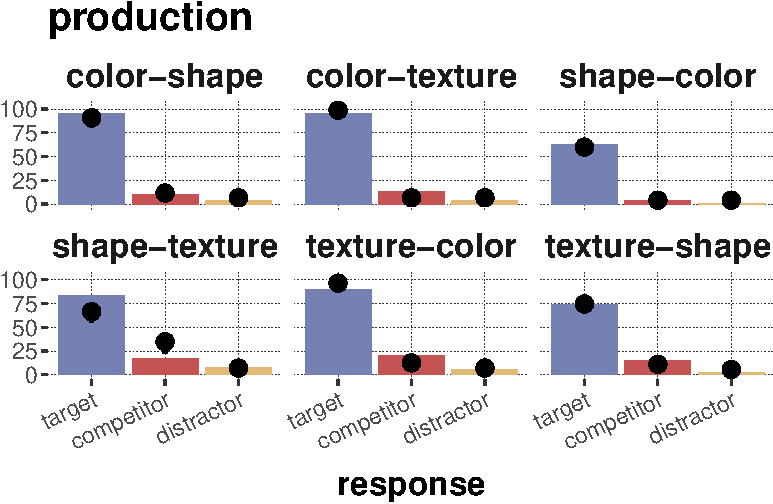
\includegraphics{00-pics/PPC-features-1.pdf}

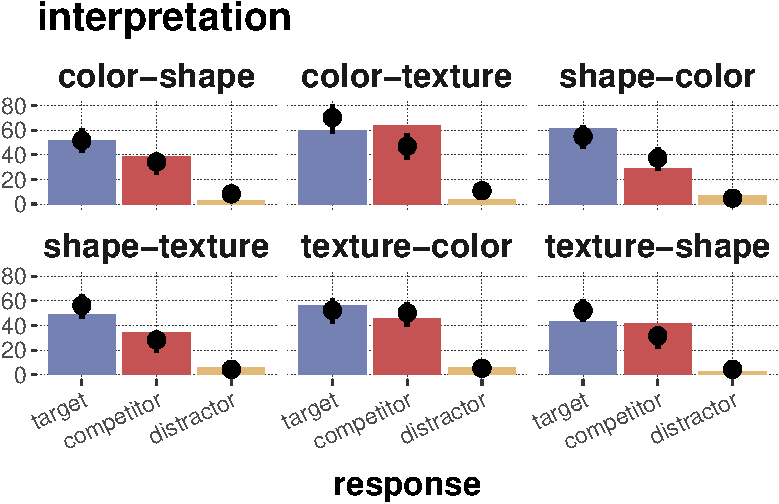
\includegraphics{00-pics/PPC-features-2.pdf}

For the production data, where there was little ground for suspecting
variation in the human data, the model's feature-wise prediction are
reasonable, with the sole expection of perhaps the
\texttt{shape-texture} condition. But for the interpretation data, there
is mild reason for diagnosing a potential systematic difference: in
conditions where the human data suggests that target and competitor
choices are roughly equal (\texttt{color-texture} and
\texttt{texture-shape}), the model still predicts that target choices
should be preferred; reversely, where the model predicts that target and
distractor choices are rather similar, the \texttt{texture-color}
condition, the human data is biased towards the target. ( {TODO: rethink
conclusion})

\hypertarget{effects-of-order-of-choice-options}{%
\subsection{Effects of order of choice
options}\label{effects-of-order-of-choice-options}}

\hypertarget{human-data-1}{%
\subsubsection{Human data}\label{human-data-1}}

Human choice counts for each order of answer alternatives are shown
below.

\begin{itemize}
\item
  for production: there is some variation but the target is consistently
  the preferred option (by a margin)
\item
  for interpretation: there are cases where the competitor is chose more
  frequently than the target
\end{itemize}

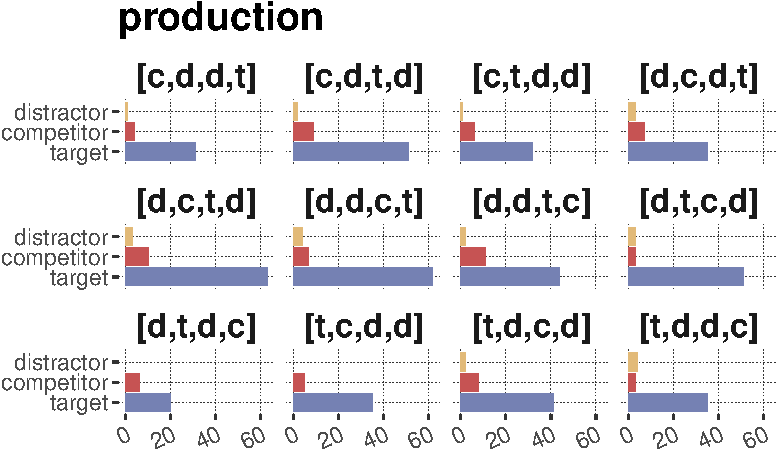
\includegraphics{00-pics/human-data-counts-per-choiceOrder-1.pdf}

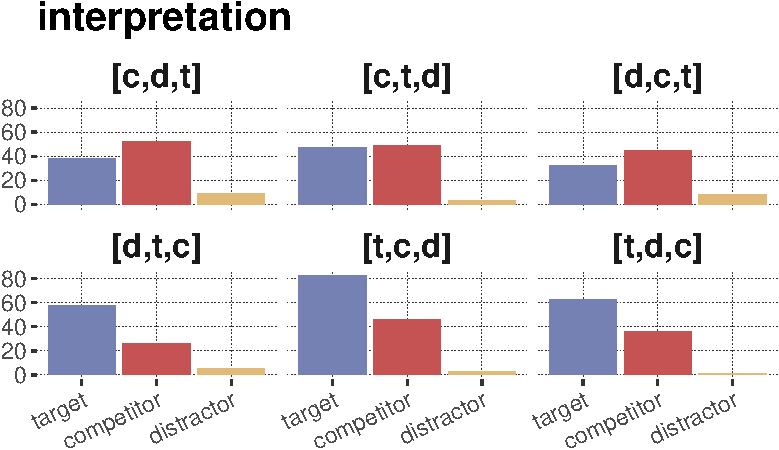
\includegraphics{00-pics/human-data-counts-per-choiceOrder-2.pdf}

BDA logistic comparing numerically highest and lowest options \ldots{}
not credibly different for production.

\begin{verbatim}
Outcome of comparing groups:
 * higher:  position == "[d,t,c,d]"
 * lower:   position == "[d,t,d,c]"
Mean 'higher - lower':  0.9518
95% HDI:  [ -0.3213 ; 2.252 ]
P('higher - lower' > 0):  0.9275
Posterior odds:  12.79
\end{verbatim}

\ldots{} but for interpretation \ldots{}

\begin{verbatim}
Outcome of comparing groups:
 * higher:  position == "[d,t,c]"
 * lower:   position == "[d,c,t]"
Mean 'higher - lower':  1.152
95% HDI:  [ 0.5446 ; 1.788 ]
P('higher - lower' > 0):  0.9998
Posterior odds:  3999
\end{verbatim}

Loo-based model comparison for interpretation against intercept-only
model shows that a model which includes order of choice options as an
explanatory factor is significantly better than an intercept-only model.

\begin{verbatim}
                           elpd_diff se_diff
fit_choice_inter             0.0       0.0
fit_choice_inter_Intercept -11.2       5.8
\end{verbatim}

We may conclude from this that there is reaonable support for the
supposition that the human interpretation data is influenced by the
order of presentation of choice alternatives.

\hypertarget{model-predictions-1}{%
\subsubsection{Model predictions}\label{model-predictions-1}}

It remains to inspect whether the model, which also seems susceptible to
choice-order, is compatible with the human data on a by choice-order
level.

The summary stats for the feature-wise model are: ( { TODO: interpret
this })

\begin{verbatim}
# A tibble: 6 x 5
  Parameter     `|95%`   mean `95%|` condition
  <chr>          <dbl>  <dbl>  <dbl> <chr>
1 alpha      0.520     0.756   1.00  production
2 epsilon    0.0610    0.0869  0.115 production
3 alpha      0.206     0.250   0.302 interpretation
4 epsilon    0.0000106 0.0374  0.106 interpretation
5 alpha      0.277     0.507   0.773 diff. prod-inter
6 epsilon   -0.0323    0.0495  0.106 diff. prod-inter
\end{verbatim}

The visual posterior predictive fits for the feature-wise
\(\alpha\epsilon\)-model for the production model is:

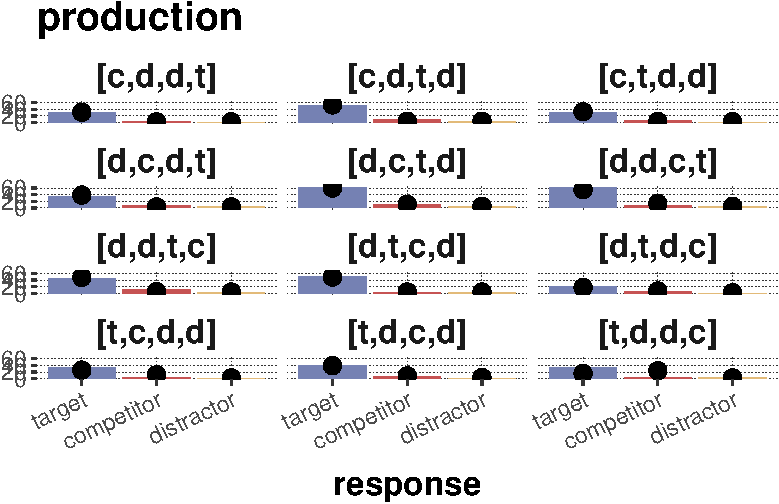
\includegraphics{00-pics/PPC-choice-1.pdf}

The posterior predictives fo the LLM-based model are decent, except for
one case: in order condition \texttt{{[}t,d,d,c{]}} the model predicts a
higher competitor choice probability, but this pattern is not supported
by the human data.

The PPC for the interpretation data is:

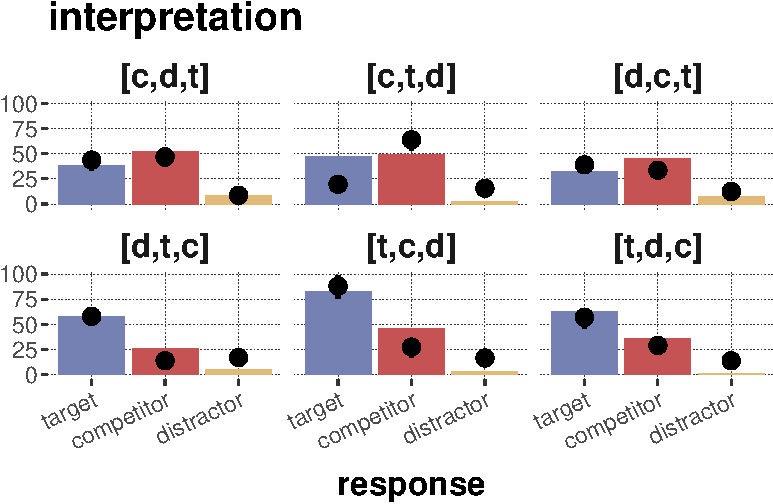
\includegraphics{00-pics/PPC-choice-interpretation-1.pdf}

Here, the model's predictions are strictly speaking off in a number of
cases (e.g., severely overpredicting the distractor choice rate), but
they are qualitatively quire remarkable. In cases where the human data
favors the competitor (top row), the model also predicts relatively
higher choice rates for the competitor, and vice versa.

\hypertarget{conclusion}{%
\section{Conclusion}\label{conclusion}}

It is not entirely ludicrous to use numerical predictions from LLMs are
part of predictive probabilistic models. But we have to be careful.
Ideally, we average out over low-level variation, such as from order of
presentation or similar ``nuisance,'' at least as long as we do not
understand what causes this variation in the predictions of models and
further research that investigates when exactly this variation accords
with empirically observed patterns.

This also implies that we should likely \emph{not} (yet) aspire to use
LLMs are models or individual- or item-level predictors.

( {TODO: rethink conclusion})

{to be continued}

\newpage
\appendix

\section{Screenshots from the online experiment with human participants}
\label{sec:scre-from-online}

Figure~\ref{fig:refgame-screenshot-production} shows a trial from the production condition, Figure~\ref{fig:refgame-screenshot-interpretation} one for the interpretation condition of the online experiment.

\begin{figure}[H]
  \centering
  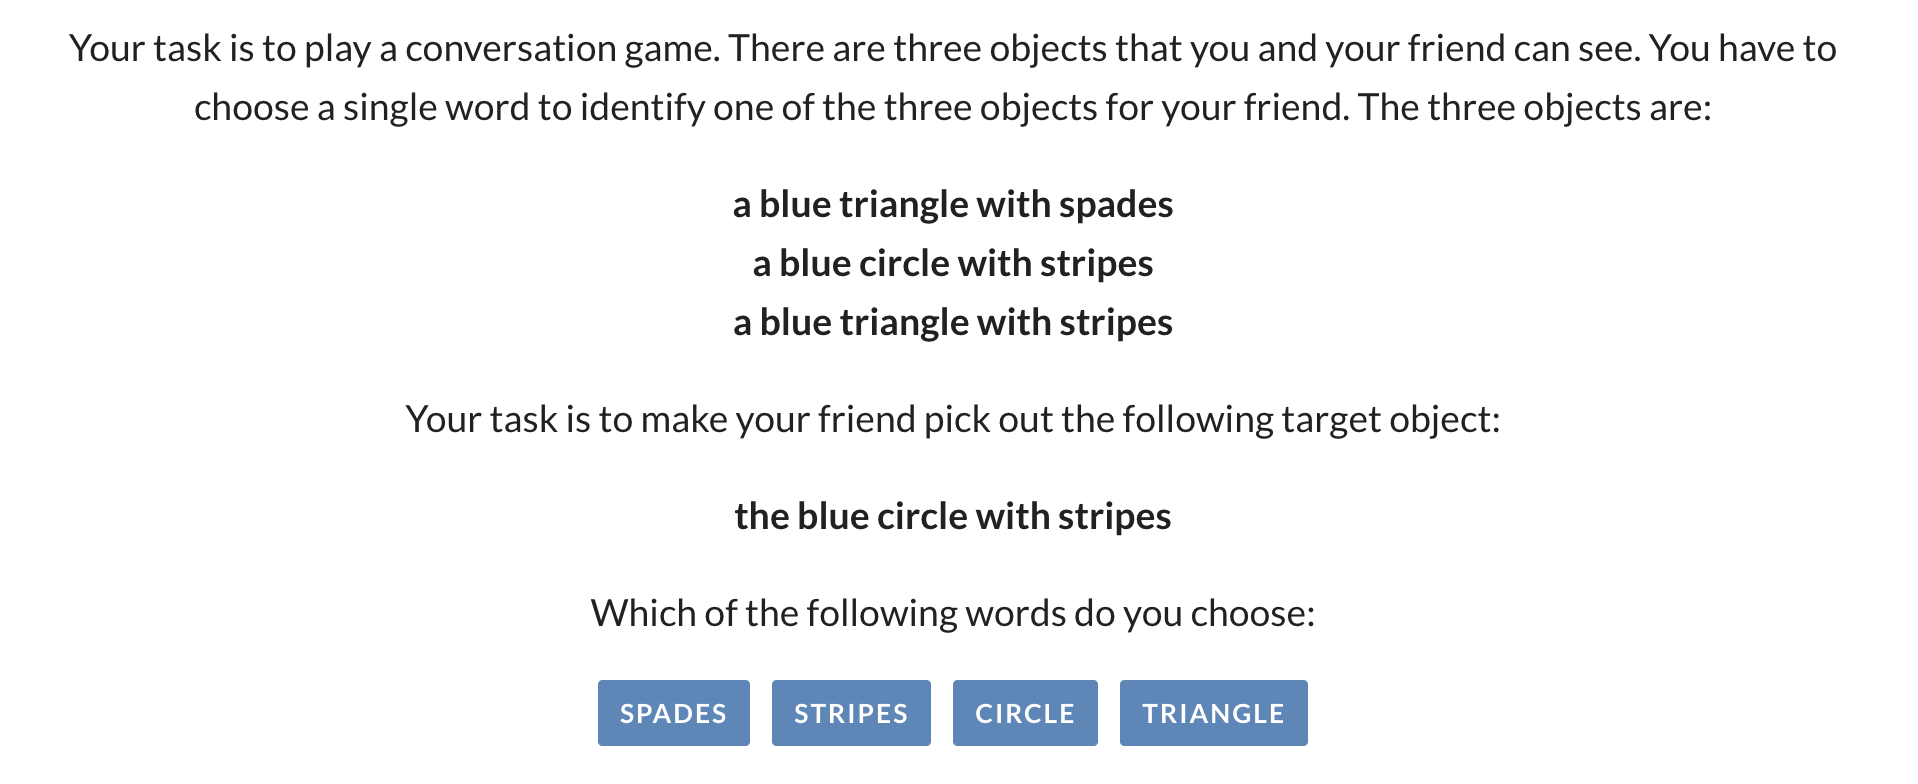
\includegraphics[width = 0.8\textwidth]{00-pics/refgame-production.png}

  \caption{Screen shot from a production trial of the online experiment.}
  \label{fig:refgame-screenshot-production}
\end{figure}

\begin{figure}[H]
  \centering
  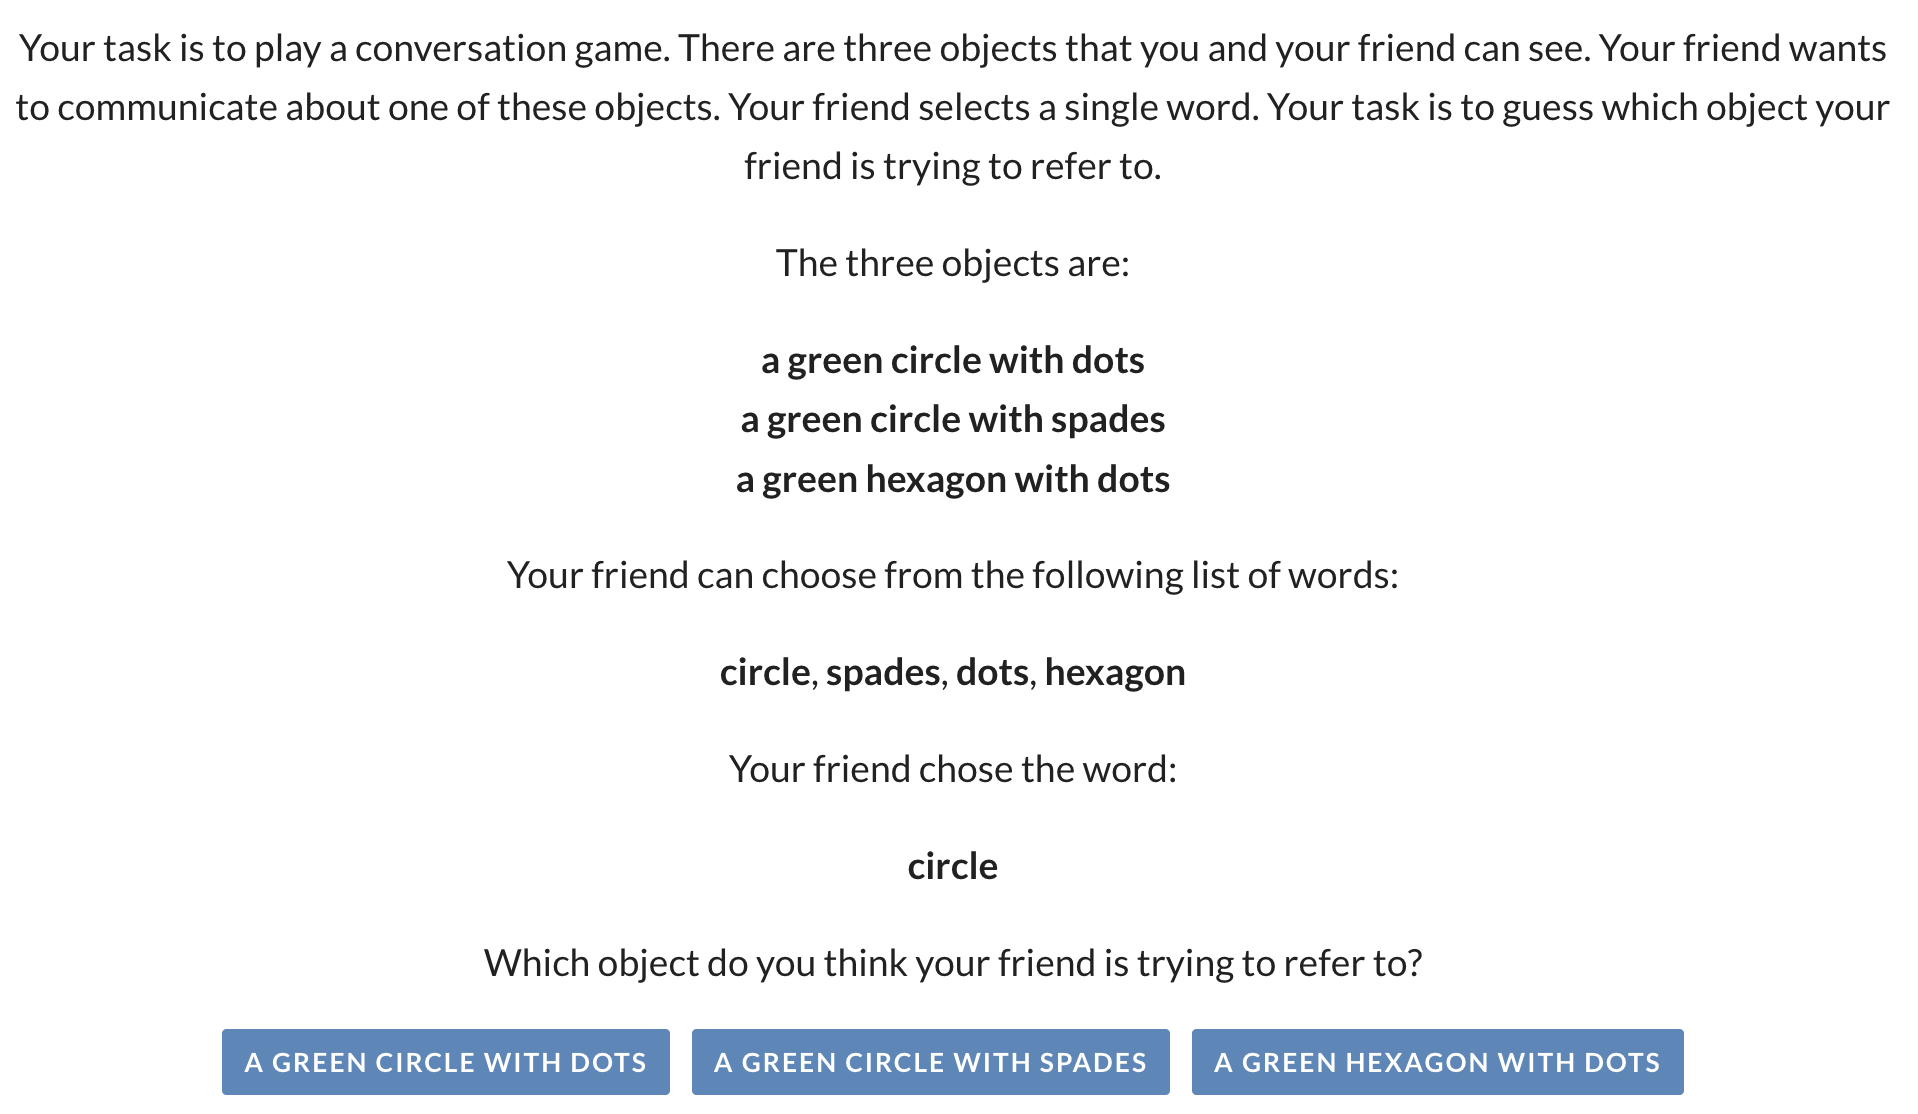
\includegraphics[width = 0.8\textwidth]{00-pics/refgame-interpretation.png}

  \caption{Screen shot from an interpretation trial of the online experiment.}
  \label{fig:refgame-screenshot-interpretation}
\end{figure}

\section{Example item for the LLM experiment}
\label{sec:examples-items-llm}

The text-based input for the LLM predictions mirrors the text in the human experiment, except that the LLM input also lists the set of all available choice options (which for the human experiment is unnecessary since this information is given by the buttons for the forced-choice selection).
For example, the task description $T_{k}$ for the item that corresponds to the production trial shown in Figure~\ref{fig:refgame-screenshot-production} is shown below (the actual input has no line breaks in the first paragraph):

\begin{verbatim}
Your task is to play a conversation game. There are three objects that
you and your friend can see. You have to choose a single word to identify
one of the three objects for your friend.

The three objects are:

a blue triangle with spades
a blue circle with stripes
a blue triangle with stripes

Your task is to make your friend pick out the following target object:

the blue circle with stripes

Which of the following words would you choose:

spades
stripes
circle
triangle

Your answer:

I would choose the word
\end{verbatim}


\printbibliography[heading=bibintoc]


\end{document}
